\RequirePackage{currfile}
\documentclass[12pt]{beamer}
\usepackage[utf8]{inputenc}
\usepackage[spanish]{babel}
\usepackage{standalone}
\usepackage{color}
\usepackage{siunitx}
\usepackage{hyperref}
%\hypersetup{colorlinks,linkcolor=,urlcolor=blue}
%\hypersetup{colorlinks,urlcolor=blue}
\usepackage{xcolor,soul}
\usepackage{etoolbox}
\usepackage{amsmath}
\usepackage{amsthm}
\usepackage{physics}
\usepackage{multicol}
\usepackage{bookmark}
\usepackage{longtable}
\usepackage{listings}
\usepackage{graphicx}
\usepackage{tikz}
\usepackage[siunitx, RPvoltages]{circuitikz}
\usetikzlibrary{arrows, patterns, matrix, backgrounds, decorations, shapes, decorations.markings, decorations.pathmorphing}
\usepackage[autostyle,spanish=mexican]{csquotes}
\usepackage[os=win]{menukeys}
\usepackage{pifont}
\usepackage{pbox}
\usepackage{caption}
\captionsetup{font=scriptsize,labelfont=scriptsize}
%\usepackage[sfdefault]{roboto}  %% Option 'sfdefault' only if the base font of the document is to be sans serif

%Sección de definición de colores
\definecolor{ao}{rgb}{0.0, 0.5, 0.0}
\definecolor{bisque}{rgb}{1.0, 0.89, 0.77}
\definecolor{amber}{rgb}{1.0, 0.75, 0.0}
\definecolor{armygreen}{rgb}{0.29, 0.33, 0.13}
\definecolor{alizarin}{rgb}{0.82, 0.1, 0.26}
\definecolor{cadetblue}{rgb}{0.37, 0.62, 0.63}
\definecolor{deepblue}{rgb}{0,0,0.5}
\definecolor{brown}{rgb}{0.59, 0.29, 0.0}
\definecolor{OliveGreen}{rgb}{0,0.25,0}


\usefonttheme[onlymath]{serif}
%Sección de definición de nuevos comandos

\newcommand*{\TitleParbox}[1]{\parbox[c]{1.75cm}{\raggedright #1}}%
\newcommand{\python}{\texttt{python}}
\newcommand{\textoazul}[1]{\textcolor{blue}{#1}}
\newcommand{\azulfuerte}[1]{\textcolor{blue}{\textbf{#1}}}
\newcommand{\funcionazul}[1]{\textcolor{blue}{\textbf{\texttt{#1}}}}
\newcommand{\ptilde}[1]{\ensuremath{{#1}^{\prime}}}
\newcommand{\ptildosargs}[2]{\ensuremath{{#1}^{\prime \, ({#2})}}}
\newcommand{\stilde}[1]{\ensuremath{{#1}^{\prime \prime}}}
\newcommand{\ttilde}[1]{\ensuremath{{#1}^{\prime \prime \prime}}}
\newcommand{\ntilde}[2]{\ensuremath{{#1}^{(#2)}}}
\renewcommand{\arraystretch}{1.5}

\newcounter{saveenumi}
\newcommand{\seti}{\setcounter{saveenumi}{\value{enumi}}}
\newcommand{\conti}{\setcounter{enumi}{\value{saveenumi}}}
\renewcommand{\rmdefault}{cmr}% cmr = Computer Modern Roman

\linespread{1.5}

\usefonttheme{professionalfonts}
%\usefonttheme{serif}
\DeclareGraphicsExtensions{.pdf,.png,.jpg}


%Sección para el tema de beamer, con el theme, usercolortheme y sección de footers
\mode<presentation>
{
  \usetheme{CambridgeUS}
  \setbeamertemplate{headline}{}
  %\useoutertheme{infolines}
  \useoutertheme{default}
  \usecolortheme{rose}
  \setbeamercovered{invisible}
  % or whatever (possibly just delete it)
  \setbeamertemplate{section in toc}[sections numbered]
  \setbeamertemplate{subsection in toc}[subsections numbered]
  \setbeamertemplate{subsection in toc}{\leavevmode\leftskip=3.2em\rlap{\hskip-2em\inserttocsectionnumber.\inserttocsubsectionnumber}\inserttocsubsection\par}
  \setbeamercolor{section in toc}{fg=blue}
  \setbeamercolor{subsection in toc}{fg=blue}
  \setbeamercolor{frametitle}{fg=blue}

  \setbeamertemplate{footline}
  %\beamertemplatenavigationsymbolsempty
}

\makeatletter
\setbeamercolor{section in foot}{bg=gray!30, fg=black!90!orange}
\setbeamercolor{subsection in foot}{bg=blue!30!yellow, fg=red}
\setbeamertemplate{footline}
{
  \leavevmode%
  \hbox{%
  \begin{beamercolorbox}[wd=.333333\paperwidth,ht=2.25ex,dp=1ex,center]{section in foot}%
    \usebeamerfont{section in foot} \insertsection
  \end{beamercolorbox}}%
  \begin{beamercolorbox}[wd=.333333\paperwidth,ht=2.25ex,dp=1ex,center]{subsection in foot}%
    \usebeamerfont{subsection in foot}  \insertsubsection
  \end{beamercolorbox}%
  \begin{beamercolorbox}[wd=.333333\paperwidth,ht=2.25ex,dp=1ex,right]{date in head/foot}%
    \usebeamerfont{date in head/foot} \insertshortdate{} \hspace*{2em}
    \insertframenumber{} / \inserttotalframenumber \hspace*{2ex} 
  \end{beamercolorbox}}%
  \vskip0pt%
\makeatother  

\makeatletter
\patchcmd{\beamer@sectionintoc}
  {\vfill}
  {\vskip\itemsep}
  {}
  {}
\makeatother

% \makeatletter
% \patchcmd{\hyper@link@}
%   {{\Hy@tempb}{#4}}
%   {{\Hy@tempb}{\ul{#4}}}
%   {}{}
% \makeatother


% Sección para el código

\definecolor{Code}{rgb}{0,0,0}
\definecolor{Keywords}{rgb}{255,0,0}
\definecolor{Strings}{rgb}{255,0,255}
\definecolor{Comments}{rgb}{0,0,255}
\definecolor{Numbers}{rgb}{255,128,0}

\DeclareCaptionFont{white}{\color{white}}
\DeclareCaptionFormat{listing}{\colorbox{gray}{\parbox{0.99\textwidth}{#1#2#3}}}
\captionsetup[lstlisting]{format=listing,labelfont=white,textfont=white}
\renewcommand{\lstlistingname}{Código}

\lstset{
basicstyle=\ttfamily,
columns=fullflexible,
breaklines=true
}

\lstdefinestyle{codigopython}{%
  language=Python,                % choose the language of the code
  %basicstyle=\footnotesize\small,       % the size of the fonts that are used for the code
  numbers=left,                   % where to put the line-numbers
  numberstyle=\scriptsize,      % the size of the fonts that are used for the line-numbers
  stepnumber=1,                   % the step between two line-numbers. If it is 1 each line will be numbered
  numbersep=5pt,                  % how far the line-numbers are from the code
  backgroundcolor=\color{white},  % choose the background color. You must add \usepackage{color}
  showspaces=false,               % show spaces adding particular underscores
  showstringspaces=false,         % underline spaces within strings
  showtabs=false,                 % show tabs within strings adding particular underscores
  frame=single,   		% adds a frame around the code
  tabsize=2,  		% sets default tabsize to 2 spaces
  captionpos=t,   		% sets the caption-position to bottom
  breaklines=true,    	% sets automatic line breaking
  breakatwhitespace=false,    % sets if automatic breaks should only happen at whitespace
  escapeinside={\#},  % if you want to add a comment within your code
  stringstyle =\color{OliveGreen},
  texcl = true,
  %otherkeywords={{as}},             % Add keywords here
  keywordstyle = \color{blue},
  commentstyle = \color{black},
  identifierstyle = \color{black},
  % literate=%
  %         {á}{{\'a}}1
  %         {é}{{\'e}}1
  %         {í}{{\'i}}1
  %         {ó}{{\'o}}1
  %         {ú}{{\'u}}1
  %
  %keywordstyle=\ttb\color{deepblue}
  %fancyvrb = true,
literate={0}{{\textcolor{red}{0}}}{1}%
            {1}{{\textcolor{red}{1}}}{1}%
            {2}{{\textcolor{red}{2}}}{1}%
            {3}{{\textcolor{red}{3}}}{1}%
            {4}{{\textcolor{red}{4}}}{1}%
            {5}{{\textcolor{red}{5}}}{1}%
            {6}{{\textcolor{red}{6}}}{1}%
            {7}{{\textcolor{red}{7}}}{1}%
            {8}{{\textcolor{red}{8}}}{1}%
            {9}{{\textcolor{red}{9}}}{1}%
            {.0}{{\textcolor{red}{.0}}}{2}% Following is to ensure that only periods
            {.1}{{\textcolor{red}{.1}}}{2}% followed by a digit are changed.
            {.2}{{\textcolor{red}{.2}}}{2}%
            {.3}{{\textcolor{red}{.3}}}{2}%
            {.4}{{\textcolor{red}{.4}}}{2}%
            {.5}{{\textcolor{red}{.5}}}{2}%
            {.6}{{\textcolor{red}{.6}}}{2}%
            {.7}{{\textcolor{red}{.7}}}{2}%
            {.8}{{\textcolor{red}{.8}}}{2}%
            {.9}{{\textcolor{red}{.9}}}{2}%
            {\ }{{ }}{1}% handle the space
        ,%
        %mathescape=true
        %escapeinside={*@}
        escapeinside={A_}{_B}
}

\title{Tema 3 - Métodos directos para EDO2}
\subtitle{Curso de Física Computacional}
\author[]{M. en C. Gustavo Contreras Mayén}
\date{28 de abril de 2020}
\begin{document}
\maketitle
\fontsize{14}{14}\selectfont
\spanishdecimal{.}
\section*{Contenido}
\frame[allowframebreaks]{\tableofcontents[currentsection, hideallsubsections]}
\section{Introducción}
\frame{\tableofcontents[currentsection, hideothersubsections]}
\subsection{Motivación}
\begin{frame}
\frametitle{Introducción}
Los problemas de Cauchy para las EDO2 se presentan en muchas áreas de la física, las ciencias aplicadas y la ingeniería, describiendo con mayor frecuencia dependencias temporales o espaciales de las cantidades continuas de interés.
\end{frame}
\begin{frame}
\frametitle{Introducción}
Por diferentes que parezcan dos de las ODE2 clásicas, a saber: la segunda ley de Newton y la ecuación de Schrödinger 1D independiente del tiempo, los métodos numéricos aplicables para su solución comparten muchas características comunes.
\end{frame}
\begin{frame}
\frametitle{Problema general de Cauchy}
Consideremos así el problema genérico de Cauchy:
\begin{align}
\dv[2]{y}{t} &= f(t, y, \ptilde{y}) \label{eq:ecuacion_12_54} \\[0.5em]
y(t_{0}) &= y_{0}, \hspace{0.5cm} \ptilde{y} (t_{0}) = \ptilde{y}_{0} \label{eq:ecuacion_12_55}
\end{align}
\end{frame}
\begin{frame}
\frametitle{Solución con serie de Taylor}
Los algoritmos desarrollados para resolverlo generalmente se derivan del método de la serie Taylor, con la primera derivada y que se propaga explícitamente junto con la solución.
\end{frame}
\begin{frame}
\frametitle{Solución con serie de Taylor}
Considerando dos valores consecutivos de la variable independiente, $t_{m}$ y $t_{m + 1}$, separados por $h = t_{m+1} - t_{m}$, y comenzando por los valores iniciales conocidos $y_{m} \equiv y (t_{m})$ e $\ptilde{y}_{m} \equiv \ptilde{y} (t_{m})$, la propagación de la solución para $t_{m + 1}$ se puede realizar con base a las expansiones de Taylor de $y$ e $\ptilde{y}$, con la segunda derivada $\stilde{y}$ determinada directamente de la EDO.
\end{frame}
\begin{frame}
\frametitle{Sistema de ecuaciones}
Las ecuaciones relevantes ordenadas en orden lógico serán:
\begin{align}
\begin{aligned}
\stilde{y}_{m} &= f(t_{m}, y_{m}, \ptilde{y}) \\[0.5em]
y_{m+1} &= y_{m} + h \, \ptilde{y}_{m} + \dfrac{1}{2} \, h^{2} \, \stilde{y}_{m} + \order{h^{3}} \\[0.5em]
\ptilde{y}_{m+1} &= \ptilde{y}_{m} + h \, \stilde{y}_{m} + \order{h^{2}}
\end{aligned}
\label{eq:eq:ecuacion_12_56}
\end{align}
\end{frame}
\begin{frame}
\frametitle{Sistema de ecuaciones}
Una característica que define a todos los algoritmos construidos en estas ecuaciones es que cada paso de propagación requiere \emph{una sola evaluación de la segunda derivada} del lado derecho de la EDO.
\end{frame}
\section{Métodos directos para EDO2}
\frame{\tableofcontents[currentsection, hideothersubsections]}
\subsection{Método de Euler para EDO2}
\begin{frame}
\frametitle{Método de Euler para EDO2}
Las implementaciones prácticas en realidad usan variantes de estas ecuaciones, ajustadas alternativamente para simplicidad, precisión o eficiencia de almacenamiento.
\\
\bigskip
La variante más simple es el \textoazul{método de Euler}, que es el equivalente para las EDO2 descrito en la presentación anterior.
\end{frame}
\begin{frame}
\frametitle{Método de Euler para EDO2}
El método de Euler esencialmente implica mantener las aproximaciones lineales en los propagadores de la posición y la velocidad:
\begin{align}
\begin{aligned}
\stilde{y}_{m} &= f(t_{m}, y_{m}, \ptilde{y}) \\[0.5em]
y_{m+1} &= y_{m} + h \, \ptilde{y}_{m} + \order{h^{2}} \\[0.5em]
\ptilde{y}_{m+1} &= \ptilde{y}_{m} + h \, \stilde{y}_{m} + \order{h^{2}}
\end{aligned}
\label{eq:eq:ecuacion_12_57}
\end{align}
\end{frame}
\begin{frame}
\frametitle{Método de Euler para EDO2}
Dado que solo usa información de $t_{m}$ (no de $t_{m + 1}$), este esquema también se conoce como \emph{aproximación de primer punto} y su ventaja obvia es la facilidad de implementación.
\end{frame}
\begin{frame}
\frametitle{Inconvenientes del método}
A pesar de su simplicidad atractiva, el método de Euler es poco recomendable debido a sus inconvenientes no despreciables:
\setbeamercolor{item projected}{bg=blue!70!black,fg=yellow}
\setbeamertemplate{enumerate items}[circle]
\begin{enumerate}
\item Con su error de truncamiento global $\order{h}$, es el esquema de solución de orden más bajo para una EDO2.
\seti
\end{enumerate}
\end{frame}
\begin{frame}
\frametitle{Inconvenientes del método}
\setbeamercolor{item projected}{bg=blue!70!black,fg=yellow}
\setbeamertemplate{enumerate items}[circle]
\begin{enumerate}
\conti
\item Debido a la rápida propagación de los errores de truncamiento, a menudo produce soluciones inestables, especialmente para sistemas oscilatorios.
\seti
\end{enumerate}
\end{frame}
\begin{frame}
\frametitle{Inconvenientes del método}
\setbeamercolor{item projected}{bg=blue!70!black,fg=yellow}
\setbeamertemplate{enumerate items}[circle]
\begin{enumerate}
\conti
\item Dado que solo usa información de $t_{m}$, la propagación de $t_{m}$ a $t_{m + 1}$ no es reversible en el tiempo (el propagador no es simétrico en $t$).
\end{enumerate}
\end{frame}
\subsection{Método Euler-Cromer}
\begin{frame}
\frametitle{El método Euler-Cromer}
El llamado \textoazul{método Euler-Cromer} usa las mismas aproximaciones de orden $\order{h}$ de la serie Taylor, pero, lo que es más importante, \emph{resuelve la inestabilidad} del método Euler.
\end{frame}
\begin{frame}
\frametitle{El método Euler-Cromer}
Las relaciones básicas se obtienen formalmente mediante la simple inversión de las ecuaciones para $\ptilde{y}_{m + 1}$ e $y_{m + 1}$, y al usar en la última, en lugar de la derivada inicial $\ptilde{y}_{m}$, el valor actualizado $\ptilde{y}_{m+1}$:
\end{frame}
\begin{frame}
\frametitle{El método Euler-Cromer}
\begin{align}
\begin{aligned}
\stilde{y}_{m} &= f(t_{m}, y_{m}, \ptilde{y}) \\[0.5em]
\ptilde{y}_{m+1} &= \ptilde{y}_{m} + h \, \stilde{y}_{m} + \order{h^{2}} \\[0.5em]
y_{m+1} &= y_{m} + h \, \ptilde{y}_{m} + \order{h^{2}}
\end{aligned}
\label{eq:eq:ecuacion_12_58}
\end{align}
\end{frame}
\begin{frame}
\frametitle{Mejora con el método Euler-Cromer}
En las implementaciones, la evaluación anterior de $\ptilde{y}_{m + 1}$ y su uso posterior en $y_{m + 1}$ permite que se asigne una sola variable de programa tanto para $\ptilde{y}_{m}$ como para $\ptilde{y}_{m + 1}$.
\end{frame}
\begin{frame}
\frametitle{Mejora con el método Euler-Cromer}
Además, con el uso de la derivada actualizada, y por lo tanto de la información de $t_{m}$ y $t_{m + 1}$, se demuestra una mejora radical en la estabilidad de la solución.
\\
\bigskip
\pause
Sin embargo, en términos de precisión de la solución, el \funcionazul{método Euler-Cromer} \emph{mantiene el mismo orden bajo} de $\order{h}$ que el método original de Euler.
\end{frame}
\subsection{Algoritmos de orden \texorpdfstring{$\order{h^{2}}$}{}}
\begin{frame}
\frametitle{Algoritmos de orden $\order{h^{2}}$}
El \textoazul{método de velocidad Verlet} considerado a continuación, pertenece a una familia de algoritmos de orden $\order{h^{2}}$ algebraicamente equivalentes, que incluye el \textoazul{método Verlet original} y el \textoazul{método Leapfrog}.
\end{frame}
\begin{frame}
\frametitle{Utilidad de los algoritmos}
En general, se emplean para resolver las ecuaciones de movimiento de Newton en simulaciones de dinámica molecular, pero también pueden usarse para resolver problemas de valores iniciales para otras EDO2.
\end{frame}
\begin{frame}
\frametitle{Utilidad de los algoritmos}
La principal diferencia entre los algoritmos \textoazul{Euler} - \textoazul{Euler-Cromer} y \textoazul{Verlet de velocidad} se refiere a mantner adicionalmente dentro de los últimos términos parabólicos en la expansión de Taylor de la solución.
\end{frame}
\subsection{El método de Verlet}
\begin{frame}
\frametitle{Ecuaciones para el método de Verlet}
Concretamente, la solución propagada puede expresarse sucesivamente como:
\begin{align*}
y_{m+1} &= y_{m} + h \, \ptilde{y}_{m} + \dfrac{1}{2} \, \stilde{y}_{m} + \order{h^{3}} = \\[0.5em]
&= y_{m} + h \left(\ptilde{y}_{m} + \dfrac{1}{2} \, h \, \stilde{y}_{m} \right) + \order{h^{3}} = \\[0.5em]
&= y_{m} + h \, \ptilde{y}_{m+1/2} + \order{h^{3}} 
\end{align*}
\end{frame}
\begin{frame}
\frametitle{El método de Verlet}
La solución $y_{m + 1}$ parece propagarse linealmente de $t_{m}$ a $t_{m + 1}$ basándose en la derivada $\ptilde{y}_{m + 1/2}$ en el intervalo medio, es decir, en $t_{m + 1/2} = t_{m} + h/2$.
\\
\bigskip
Desde una perspectiva diferente, $\ptilde{y}_{m + 1/2}$ puede considerarse como la primera derivada promedio durante el intervalo $[t_{m}, t_{m + 1}]$.
\end{frame}
\begin{frame}
\frametitle{El método de Verlet}
La solución propagada $y_{m + 1}$ sustituida en la EDO determina la segunda derivada $\stilde{y}_{m + 1}$ en el extremo del intervalo, que a su vez, también permite la propagación de la primera derivada $\ptilde{y}_{m + 1/2}$ hasta $t_{m + 1}$.
\end{frame}
\begin{frame}
\frametitle{El método de Verlet}
La secuencia de algoritmos de las fórmulas de propagación del \textoazul{método Verlet de velocidad} finalmente toma la forma:
\begin{align}
\begin{aligned}
\ptilde{y}_{m+1/2} &= \ptilde{y}_{m} + \dfrac{1}{2} \, h \, \stilde{y}_{m} + \order{h^{2}} \\[0.5em]
y_{m+1} &= y_{m} +  h \, \ptilde{y}_{m+1/2} + \order{h^{3}} \\[0.5em]
\stilde{y}_{m+1} &= f(t_{m+1}, y_{m+1}, \ptilde{y}_{m+1/2}) \\[0.5em]
\ptilde{y}_{m+1} &= \ptilde{y}_{m+1/2} + \dfrac{1}{2} \, h \, \stilde{y}_{m+1} + \order{h^{2}}
\end{aligned}
\label{eq:ecucacion_12_59}
\end{align}
\end{frame}
\begin{frame}
\frametitle{Ventaja del método de Verlet}
Además de garantizar la precisión de orden $\order{h^{2}}$ (superior en un orden sobre los métodos de \textoazul{Euler} y \textoazul{Euler-Cromer}, el \textoazul{método de Verlet de velocidad} también se destaca por la estabilidad y los pequeños requisitos de almacenamiento facilitados por la posibilidad algorítmica y computacional de que todas las cantidades se sobrescriban a lo largo de la propagación.
\end{frame}
\begin{frame}
\frametitle{Consideración importante}
Sin embargo, se debe enfatizar un aspecto que requiere atención especial: la segunda derivada $\stilde{y}_{m+1}$ determinada en un paso es necesaria no solo para propagar la primera derivada $\ptilde{y}_{m+1/2}$ durante la segunda mitad del intervalo, de $t_{m+1/2}$ a $t_{m}$, sino también para avanzar $\ptilde{y}_{m+1}$ durante la primera mitad del siguiente paso, de $t_{m+1}$ a $t_{m+3/2}$.
\end{frame}
\begin{frame}
\frametitle{Consideración importante}
Por esta razón, junto con $y_{m + 1}$ e $\ptilde{y}_{m + 1}$, también, la segunda derivada $\stilde{y}_{m + 1}$ debe guardarse para usarse en el siguiente paso.
\end{frame}
\subsection*{Implementación del código}
\begin{frame}
\frametitle{El código en \python}
A continuación se presenta una propuesta de código para los métodos de \textoazul{Euler}, \textoazul{Euler-Cromer} y \textoazul{Verlet de velocidad}, que resuelven una EDO2 de valores iniciales.
\end{frame}
\begin{frame}[fragile]
\frametitle{Método de Euler}
\begin{lstlisting}[caption=Método de Euler para EDO2, style=codigopython]
def EulerA_1_B(t, ht, y, dy, Func):
    dA_2_By = Func(t, y, dy)

    y  += ht * dy
    dy += ht * dA_2_By
    return (y, dy)
\end{lstlisting}
\end{frame}
\begin{frame}[fragile]
\frametitle{Método de Euler-Cromer}
\begin{lstlisting}[caption=Método de Euler-Cromer para EDO2, style=codigopython]
def EulerCromerA_1_B(t, ht, y, dy, Func):
    dA_2_By = Func(t, y, dy)

    dy += ht * dA_2_By
    y  += ht * dy
    return (y, dy)
\end{lstlisting}
\end{frame}
\begin{frame}[allowframebreaks, fragile]
\frametitle{Método de Verlet de velocidad}
\begin{lstlisting}[caption=Método de Verlet de velocidad para EDO2, style=codigopython]
def VerletA_1_B(t, ht, y, dy, dA_2_By, Func):
    htA_2_B = 0.5e0 * ht
    dy += htA_2_B * dA_2_By
    y  += ht  * dy

    dA_2_By = Func(t, y, dy)

    dy += htA_2_B * dA_2_By
    return (y, dy, dA_2_By)
\end{lstlisting}
\end{frame}
\subsection*{Ejemplo práctico: 2a. ley de Newton}
\begin{frame}
\frametitle{Ejemplo práctico}
Teniendo en cuenta la importancia práctica de los problemas de valores iniciales para la ecuación de movimiento de Newton:
\begin{align*}
m \, \dv[2]{\vb{r}}{t} =  \vb{F} (t, \vb{r}, \vb{v}) \hspace{1cm} \vb{r}(t_{0}) = \vb{r}_{0}, \hspace{0.5cm} \vb{v}(t_{0}) = \vb{v}_{0}
\end{align*}
donde $m$ es la masa, $\vb{r}$ y $\vb{v}$ son la posición y velocidad, $\vb{F}$ es la fuerza actuando en el objeto.
\end{frame}
\begin{frame}
\frametitle{Algoritmo de Verlet}
El algoritmo de Verlet se expresa por
\begin{align}
\begin{aligned}
\vb{r}_{m+1/2} &= \vb{v}_{m} + (h/2) \, \vb{a}_{m} \\[0.25em]
\vb{r}_{m+1} &= \vb{r} + h \, \vb{v}_{m+1/2} \\[0.25em]
\vb{a}_{m+1} &= (1/m) \, \vb{F}(t_{m+1}, \vb{r}_{m+1}, \vb{v}_{m+1/2}) \\[0.5em]
\vb{v}_{m+1} &= \vb{m}_{1/2} + (h/2) \, \vb{a}_{m+1}
\end{aligned}
\label{eq:ecuacion_12_60}
\end{align}
\end{frame}
\begin{frame}
\frametitle{Algortimo de Verlet}
En la primera etapa de cada paso de propagación, la velocidad $\vb{v}$ se cambia al intervalo medio $(\vb{v}_{m + 1/2})$ y la posición $\vb{r}$, hasta el final del intervalo de tiempo $(\vb{r}_{m + 1})$.
\\
\bigskip
La fuerza $\vb{F}$ que actúa sobre la partícula, calculada con la nueva posición, determina la aceleración correspondiente $(\vb{a}_{m + 1})$.
\end{frame}
\begin{frame}
\frametitle{Algortimo de Verlet}
En la segunda etapa, la velocidad del intervalo medio (también considerada como velocidad promedio sobre $[t_{m}, t_{m + 1}]$ se propaga hasta el final del intervalo de tiempo $(\vb{v}_{m + 1})$, completando la información dinámica en el cuerpo móvil para $(t_{m + 1})$.
\end{frame}
\begin{frame}
\frametitle{Implementación en dos dimensiones}
La implementación en dos dimensiones $(2D)$ de las relaciones de propagación (ec. \ref{eq:ecuacion_12_60}) se puede realizar, por ejemplo, para describir objetos que evolucionan a lo largo de órbitas planas.
\end{frame}
\begin{frame}
\frametitle{Implementación en dos dimensiones}
La variante del algortimo de Verlet en tres dimensiones $(3D)$ generaliza el algoritmo a un sistema de $n$ partículas que interactúan por pares y muestra las características principales de los propagadores utilizados actualmente en simulaciones de dinámica molecular a gran escala.
\end{frame}
\begin{frame}
\frametitle{Implementación de los códigos}
Como se ha mencionado en las dos diapositivas anteriores, es posible implementar el algoritmo de Verlete en $2D$ y $3D$, para resolver problemas muy específicos, que pudieran revisarse en un Seminario de Temas Selectos, para profundizar su estudio. En nuestro curso nos quedamos con la implementación en $1D$.
\end{frame}
\subsection*{Revisión de la estabilidad}
\begin{frame}
\frametitle{Revisión de la estabilidad}
Con la finalidad de demostrar la estabilidad de los métodos de \textoazul{Euler}, \textoazul{Euler-Cromer}, \textoazul{Verlet de velocidad}, ocuparemos el problema del péndulo no lineal que se revisó en la presentación anterior.
\end{frame}
\begin{frame}
\frametitle{Ocupando los algoritmos}
En el código para este problema utilizamos los métodos mencionados.
\\
\bigskip
En el caso de la función \funcionazul{Verlet1}, se necesita declarar e inicializar adicionalmente en el programa principal una variable \funcionazul{d2y}, para almacenar la segunda derivada entre llamadas a \funcionazul{Verlet1}.
\end{frame}
\begin{frame}[allowframebreaks, fragile]
\frametitle{Código}
\begin{lstlisting}[caption=Código para el método Euler-Cromer, style=codigopython]
import numpy as np
from Metodos_Directos import EulerCromerA_1_B

g = 9.81e0

def Func(t, u, v):
    return -g/l * np.sin(u) - k * v

l = 1e0
k = 0e0
uA_0_B = 0.5e0*np.pi
duA_0_B = 0e0
tmax = 20e0
ht = 0.01e0

salida = open("pendulo_euler_cromer.txt","w")
salida.write("t \t u \t du\n")

t = 0e0
u = uA_0_B; du = duA_0_B

salida.write(("{0:10.5f} \t {1:10.5f} \t {2:10.5f}\n").format(t, u, du))

while (t+ht <= tmax):
    (u, du) = EulerCromerA_1_B(t, ht, u, du, Func)
    t += ht

    salida.write(("{0:10.5f} \t {1:10.5f} \t {2:10.5f}\n").format(t, u, du))

salida.close()
\end{lstlisting}
\end{frame}
\begin{frame}
\frametitle{Gráfica obtenida}
Luego de incorporar una rutina de graficación con los datos que se enviaron al archivo de texto, obtenemos la siguiente gráfica:
\end{frame}
\begin{frame}
\frametitle{Gráfica obtenida}
\begin{figure}[h!]
    \centering
    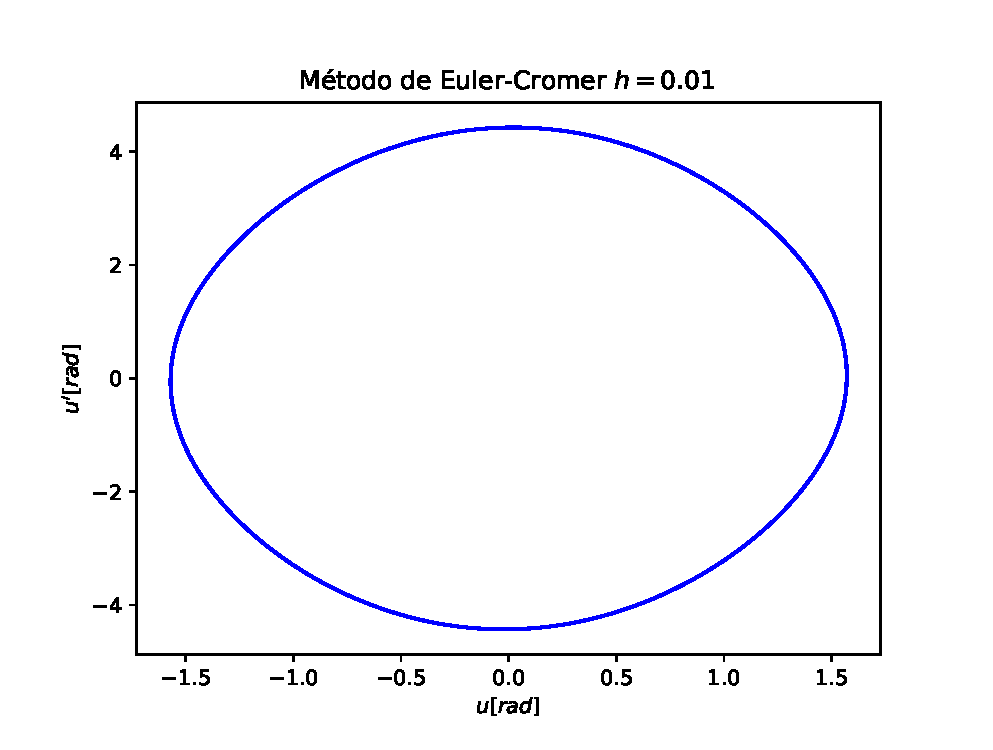
\includegraphics[scale=0.6]{Imagenes/metodo_EDO2_Euler_Cromer_01.eps}
    \caption{Solución al problema del péndulo no lineal mediante el método de Euler-Cromer.}
    \label{fig:figura_12_EDO2_01}
\end{figure}
\end{frame}
\begin{frame}
\frametitle{Comparación entre los métodos}
Como habíamos indicado previamente, nos interesa comparar los resultados de la estabilidad con los métodos, por lo que como \textbf{Ejercicio a cuenta}: deberás de realizar el ajuste necesario en el código para obtener las gráficas con el \textoazul{método de Euler} con $h=0.01$, el \textoazul{método Euler-Cromer} con $h=0.1$, y el \textoazul{método de Verlet} con $h=0.01$ y presentar las respectivas gráficas.
\end{frame}
\begin{frame}
\frametitle{Comparación entre los métodos}
\begin{columns}[t]
\column{.5\textwidth}
\centering
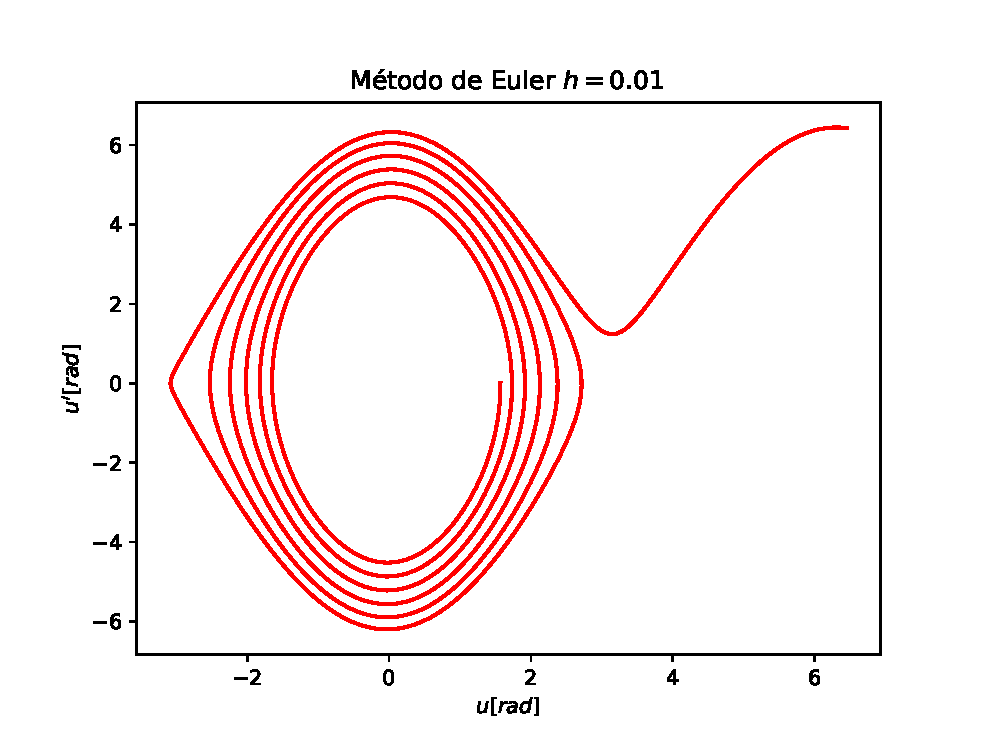
\includegraphics[width=5cm,height=3.5cm]{Imagenes/metodo_EDO2_Euler_01.eps}\\
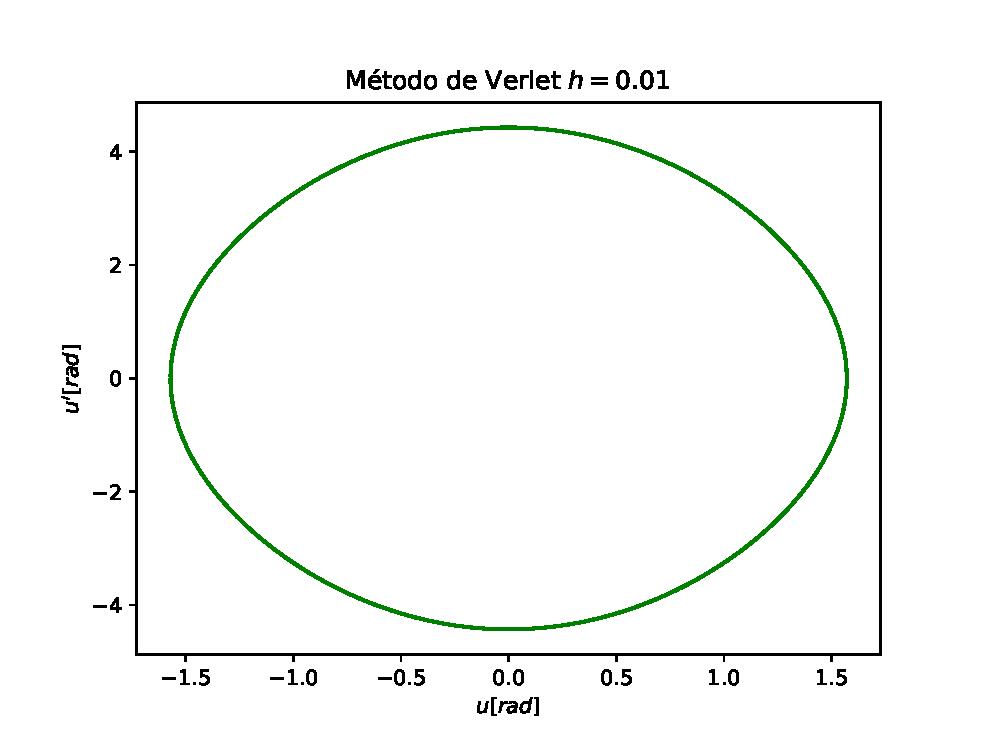
\includegraphics[width=5cm,height=3.5cm]{Imagenes/metodo_EDO2_Verlet_01.eps}
\column{.5\textwidth}
\centering
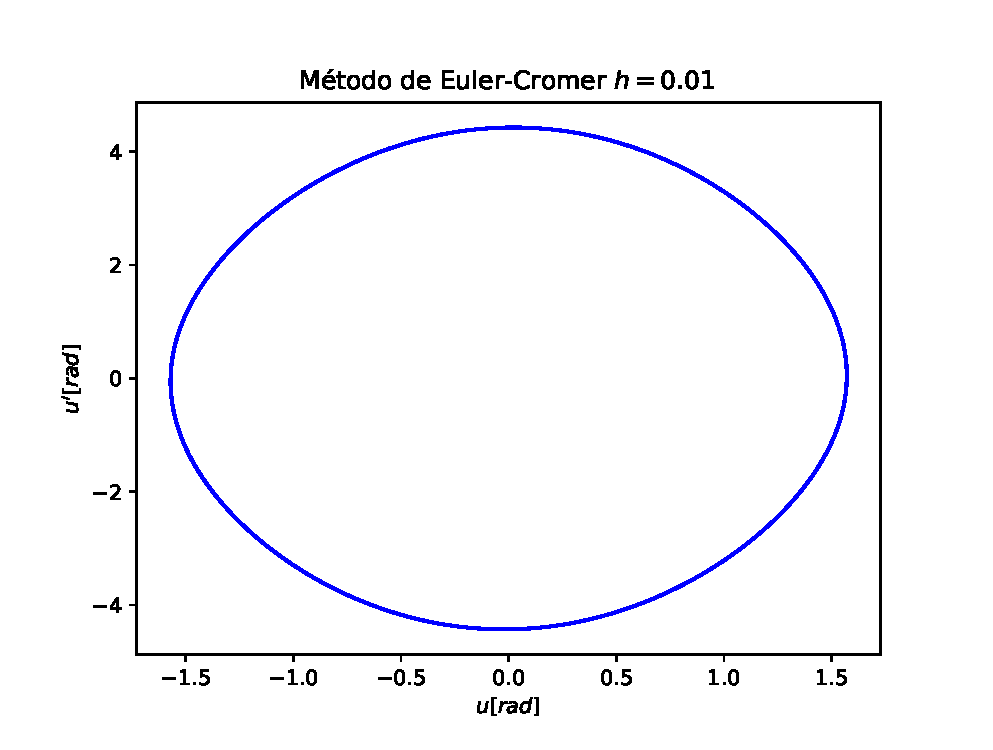
\includegraphics[width=5cm,height=3.5cm]{Imagenes/metodo_EDO2_Euler_Cromer_01.eps}\\
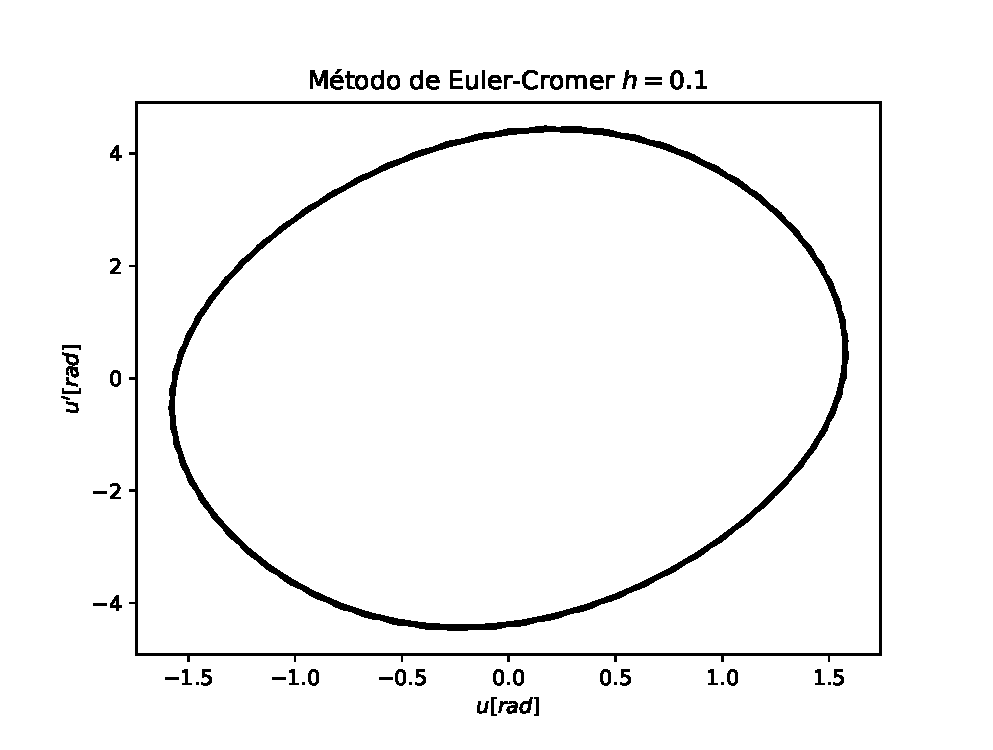
\includegraphics[width=5cm,height=3.5cm]{Imagenes/metodo_EDO2_Euler_Cromer_02.eps}
\end{columns}
\end{frame}
\begin{frame}
\frametitle{Interpretación}
En principio, en ausencia del coeficiente de arrastre $(k = 0)$, un propagador estable debería producir una trayectoria cerrada en el espacio de fase del péndulo.
\end{frame}
\begin{frame}
\frametitle{Interpretación}
Desde la gráfica superior izquierda de la diapositiva anterior, se puede ver que el \textoazul{método de Euler} (rutina \funcionazul{Euler1}) es notablemente inestable incluso para un tamaño de paso tan pequeño como $h = 0.01$.
\end{frame}
\begin{frame}
\frametitle{Interpretación}
En contraste y a pesar de ser igualmente preciso de primer orden, el \textoazul{método Euler-Cromer} (rutina \funcionazul{EulerCromer1}) permanece estable incluso para un tamaño de paso de $10$ veces $(h = 0.1)$ (gráfica arriba a la derecha y abajo a la derecha).
\\
\bigskip
De hecho, la trayectoria es cerrada, por lo tanto estable, aunque considerablemente distorsionada, por lo tanto inexacta.
\end{frame}
\begin{frame}
\frametitle{Interpretación}
En cuanto al \textoazul{método de Verlet de velocidad} (rutina \funcionazul{Verlet1}), su precisión superior $\order{h^{2}}$ genera una trayectoria estable y sin distorsiones incluso para tamaños de pasos para los cuales el \textoazul{método Euler-Cromer} claramente no es preciso.
\end{frame}
\section{Usando \python{} para resolver las EDO}
\frame{\tableofcontents[currentsection, hideothersubsections]}
\subsection{Antes de usar la librería}
\begin{frame}
\frametitle{Usando \python{} para resolver las EDO}
Un sistema de EDO es usualmente formulado en forma estándar antes de ser resuelto numéricamente con \python. La forma estándar es:
\begin{align*}
\ptilde{y} = f(y, t)
\end{align*}
donde
\begin{align*}
y = [y_{1}(t), y_{2}(t), \ldots, y _{n}(t)]
\end{align*}
y $f$ es una función que determina las derivadas de la función $y_{i}(t)$.
\end{frame}
\begin{frame}
\frametitle{Usando \python{} para resolver las EDO}
Para resolver la EDO necesitamos conocer la función \funcionazul{f} y una condición inicial, \funcionazul{y(0)}.
\\
\medskip
Nótese que para una EDO de orden superior siempre pueden trasformarse en esta forma introduciendo nuevas variables para las derivadas intermedias.
\end{frame}
\subsection{La función \texttt{odeint}}
\begin{frame}
\frametitle{La función \texttt{scipy.integrate.odeint}}
Dentro del paquete \funcionazul{scipy} y en el módulo \funcionazul{integrate} tenemos disponible la función \funcionazul{odeint}, que integra un sistema de EDO dado por
\begin{align*}
\dv{y}{t} = \text{ func}(y, t_{0}, ...)
\end{align*}
donde $y$ puede ser un vector.
\end{frame}
\begin{frame}[fragile]
\frametitle{La sintaxis para \texttt{odeint}}
La sintaxis básica para utilizar la función es la siguiente:
\\
\bigskip
\verb|odeint(func, y0, t, args=())|
\end{frame}
\begin{frame}
\frametitle{Los argumentos de \texttt{odeint}}
Los argumentos mínimos son los siguientes:
\setbeamercolor{item projected}{bg=yellow!80!black,fg=black}
\setbeamertemplate{enumerate items}[circle]
\begin{enumerate}[<+->]
\item \funcionazul{func} : Es la función que se manda llamar $(y, t_{0}, ...)$ Calcula la derivada de $y$ en $t_{0}$.
\item \funcionazul{y0} : Tipo arreglo. Condición inicial de $y$, puede ser un vector.
\seti
\end{enumerate}
\end{frame}
\begin{frame}
\frametitle{Los argumentos de \texttt{odeint}}
\setbeamercolor{item projected}{bg=yellow!80!black,fg=black}
\setbeamertemplate{enumerate items}[circle]
\begin{enumerate}[<+->]
\conti
\item \funcionazul{t} : Tipo arreglo. Una secuencia de puntos temporales en los cuales se va a resolver para la variable $y$. La condición inicial debe de ser el primer elemento de esta secuencia.
\item \funcionazul{args} : Tipo tupla opcional. Argumentos extra para pasar a la función.
\end{enumerate}
\end{frame}
\begin{frame}
\frametitle{Lo que devuelve la función \textbf{odeint}}
La función \funcionazul{odeint} devuelve una serie de elementos, el principal es:
\\
\medskip
\funcionazul{y} : Tipo arreglo.
\\
\medskip
Que es un arreglo bidimensional del tamaño \texttt{shape (len(t), len(y0))} que contiene los valores de \funcionazul{y} para cada punto temporal \funcionazul{t}, con la condición inicial \funcionazul{y0} en el primer renglón.
\end{frame}
\begin{frame}
\frametitle{Usando la función \texttt{odeint}}
Una vez definida la función \funcionazul{F} y el arreglo  \funcionazul{y0}, podemos usar la función \funcionazul{odeint}:
\begin{align*}
y_{t} = \text{\texttt{odeint}}(F, y_{0}, t)
\end{align*}
Nótese que contiene el mínimo de argumentos para la función, no es mala idea de que revisen en la documentación oficial de \python, los demás argumentos que se pueden ocupar.
\end{frame}
\section{Ejercicios con \texttt{odeint}}
\frame{\tableofcontents[currentsection, hideothersubsections]}
\subsection{Péndulo con fricción}
\begin{frame}
\frametitle{Ejercicio 1 - Péndulo con fricción}
La \textoazul{EDO2} para el ángulo $\theta$ de un péndulo que se desplaza bajo la acción de la gravedad y con fricción, se puede escribir como
\begin{align}
\ddot{\theta} +  b \: \dot{\theta} +  c \: \sin \theta = 0
\end{align}
donde $b$ y $c$ son constantes positivas.
\end{frame}
\begin{frame}
\frametitle{Solución al Ejercicio 1}
Para resolver el problema con la función \funcionazul{odeint} debemos convertir la EDO2 a un sistema de \textoazul{EDO1}.
\\
\bigskip
Definiendo la velocidad angular $\omega (t) = \dot{\theta}$, se obtiene el sistema
\begin{center}
\begin{align*}
\dot{\theta} &= \omega \\
\dot{\omega} &= -b \, \omega - c \, \sin(\theta)
\end{align*}
\end{center}
\end{frame}
\begin{frame}[fragile]
\frametitle{Solución al ejercicio}
Sea el vector $y =  [\theta, \omega]$. Así la función que usaremos en \python{} queda como
\begin{lstlisting}[caption=Función a integrar para el problema del péndulo, style=codigopython]
def F(y, t, b, c):
    theta, omega = y
    dydt = [omega, -b * omega - c * np.sin(theta)]
    return dydt
\end{lstlisting}
\end{frame}
\begin{frame}
\frametitle{Valores de las constantes}
Consideramos que las constantes $b$ y $c$ son:
\begin{align*}
b &= 0.25 \\
c &= 5.0
\end{align*} 
\end{frame}
\begin{frame}
\frametitle{Condiciones inciales}
Para las condiciones iniciales, supongamos que el péndulo está muy cerca de la vertical con $\theta(0) = \pi - 0.1$, y que está en reposo, por lo que $\omega(0) = 0$.
\\
\bigskip
Entonces, el vector de las condiciones iniciales queda como
\begin{align*}
y0 =  [\pi - 0.1 , \; 0.0] 
\end{align*}
\end{frame}
\begin{frame}
\frametitle{Secuencia temporal}
Generamos una secuencia de $101$ puntos temporales en el intervalo $0 \leq t \leq 10$, por lo que nuestro arreglo de tiempo es:
\begin{align*}
t =  \text{\texttt{np.linspace}}(0., \; 10., \; 101)
\end{align*}
\end{frame}
\begin{frame}[fragile]
\frametitle{Solución con \texttt{odeint}}
Usamos la función \funcionazul{odeint} para la solución; el paso de los parámetros $b$ y $c$ a \funcionazul{F}, se hace a través de \funcionazul{args}:
\begin{lstlisting}[caption=Solución al problema del péndulo con odeint, style=codigopython]
from scipy.integrate import odeint

sol = odeint(F, yA_0_B, t, args=(b, c))
\end{lstlisting}
\end{frame}
\begin{frame}
\frametitle{Soluciones en gráficas}
Se presentarán dos gráficas a partir de la solución:
\setbeamercolor{item projected}{bg=blue!70!black,fg=yellow}
\setbeamertemplate{enumerate items}[circle]
\begin{enumerate}[<+->]
\item Una gráfica que nos indique el tanto la velocidad como el desplazamiento angular.
\item Un diagrama de fase el péndulo.
\end{enumerate}
\textbf{Ejercicio a cuenta: incluir la rutina de graficación  y enviar las imágenes obtenidas, éstas se deben de obtener en una ejecución.}
\end{frame}
\begin{frame}[plain, allowframebreaks, fragile]
\frametitle{Código completo}
\begin{lstlisting}[caption=Función a integrar, style=codigopython]
from scipy.integrate import odeint
import matplotlib.pyplot as plt
import numpy as np

def F(y, t, b, c):
    theta, omega = y
    dydt = [omega, -b * omega - c * np.sin(theta)]
    return dydt

b = 0.25
c = 5.0

yA_0_B =  [np.pi - 0.1, 0.0]

t = np.linspace(0., 10., 101)

sol = odeint(F, yA_0_B, t, args=(b, c))
\end{lstlisting}
\end{frame}
\begin{frame}[plain]
\frametitle{Gráficas de la solución}
La primera gráfica representa la posición y la velocidad angular del péndulo.
\begin{figure}[h!]
    \centering
    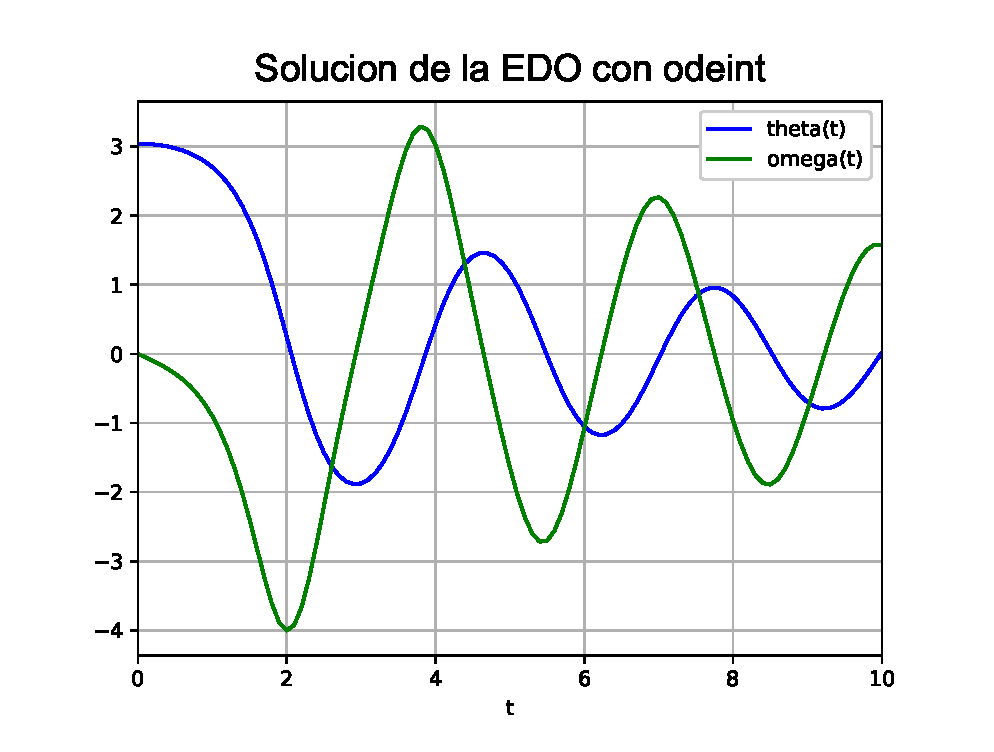
\includegraphics[scale=0.5]{Imagenes/sol_odeint_01.eps}
\end{figure}
\end{frame}
\begin{frame}[plain]
\frametitle{Gráfica del espacio fase}
\begin{figure}[h!]
    \centering
    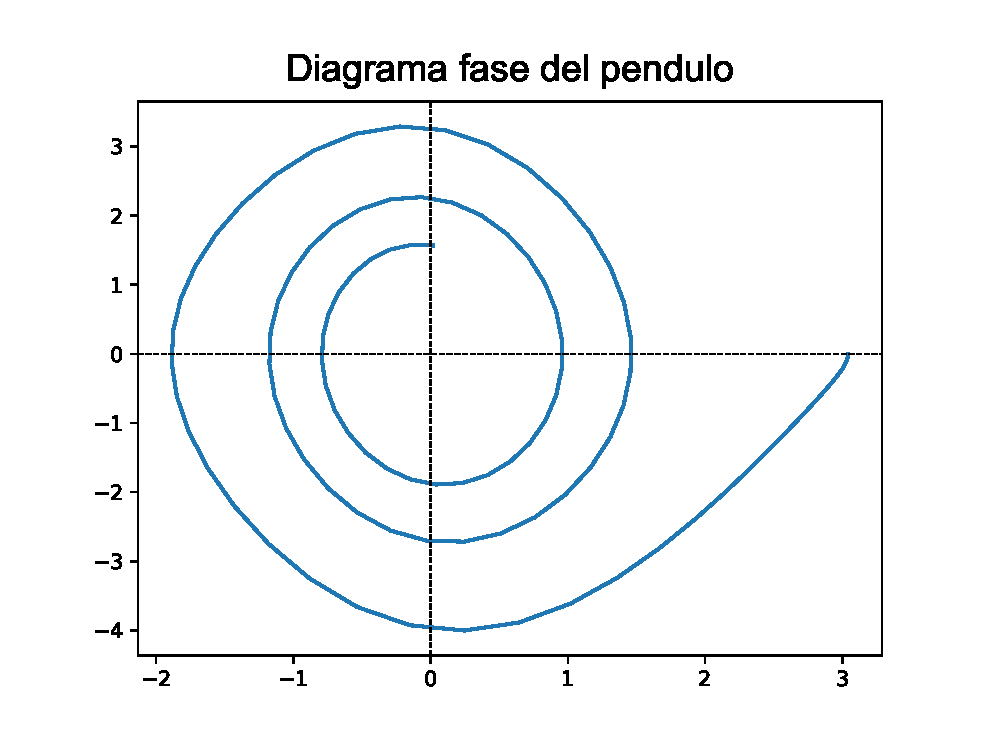
\includegraphics[scale=0.5]{Imagenes/sol_odeint_02.eps}
\end{figure}
\end{frame}
\begin{frame}
\frametitle{Gráfica del espacio fase}
La segunda gráfica representa el espacio fase, una de las interpretaciones es que hay un atractor debido a la fricción en el péndulo; la trayectoria no es cerrada y por tanto, hay pérdida de la energía.
\end{frame}
\subsection{Oscilador amortiguado}
\begin{frame}
\frametitle{Ejercicio 2 - Oscilador amortiguado}
La ecuación de movimiento para el oscilador amortiguado es:
\begin{align*}
\dv[2]{x}{t} + 2 \, \zeta \,  \omega_{0} \, \dv{x}{t} + \omega_{0}^{2} \, x = 0
\end{align*}
donde $x$ es la posición del oscilador, $\omega_{0}$ la frecuencia, y $\zeta$ es el factor de amortiguamiento.
\end{frame}
\begin{frame}
\frametitle{Re-escribiendo la EDO}
Para escribir esta \textoazul{EDO2} en la forma estándar, introducimos $p = \dv*{x}{t}$
\begin{align*}
\dv{p}{t} &= - 2 \, \zeta \, \omega_{0} \, p - \omega^{2} \, x \\[0.5em]
\dv{x}{t} &= p
\end{align*}
\end{frame}
\begin{frame}
\frametitle{Usando los argumentos}
Veremos con este ejemplo, la versatilidad de pasar argumentos extras a la función, que representan los \emph{diferentes valores del factor de amortiguamiento}.
\end{frame}
\begin{frame}
\frametitle{Usando argumentos}
De tal manera que en una sola ejecución del código, podemos \enquote{pasar} los valores, de otra manera, tendríamos que realizar una primera ejecución del código, para luego modificar a mano el valor del factor de amortiguamiento y volver a ejecutar el código.
\end{frame}
\begin{frame}
\frametitle{Usando argumentos}
Como consecuencia de los argumentos extra, necesitamos pasar dos argumentos clave \funcionazul{args} a la función \funcionazul{odeint}.
\\
\bigskip
El primero es el arreglo:
\begin{align*}
\zeta = 0.0, 0.2, 1.0, 5.0
\end{align*}
Y el segundo es \funcionazul{w0}. Los argumentos \funcionazul{args} siempre deben de darse en una \emph{tupla}.
\end{frame}
\begin{frame}[plain, allowframebreaks, fragile]
\frametitle{Código para resolver el problema}
\begin{lstlisting}[caption=Código completo para el problema del oscilador, style=codigopython]
from scipy.integrate import odeint
from numpy import zeros, array, linspace, pi

def F(y, t, zeta, wA_0_B):
    F = zeros(2, dtype='floatA_64_B')
    F[0] = y[1]
    F[1] = -2 * zeta * wA_0_B * y[1] - wA_0_B**2 * y[0]
    return F    

yA_0_B = array([1.0, 0.0])

t = linspace(0.0, 5.0, 500)
wA_0_B = 2 * pi * 1.0

yA_1_B = odeint(F, yA_0_B, t, args=(0.0, wA_0_B))
yA_2_B = odeint(F, yA_0_B, t, args=(0.2, wA_0_B))
yA_3_B = odeint(F, yA_0_B, t, args=(1.0, wA_0_B))
yA_4_B = odeint(F, yA_0_B, t, args=(5.0, wA_0_B))
\end{lstlisting}
\end{frame}
\begin{frame}
\frametitle{Resultado gráfico}
\textbf{Ejrecicio a cuenta:} Nuevamente hay que incluir una rutina de graficación para obtener en una sola imagen el resultado obtenido en cada solución.
\\
\bigskip
Toma en cuenta de que en estos ejercicios, no estamos enviando a un archivo los datos de las soluciones.
\end{frame}
\begin{frame}[plain]
\frametitle{Gráfica con las soluciones}
\begin{figure}
    \centering
    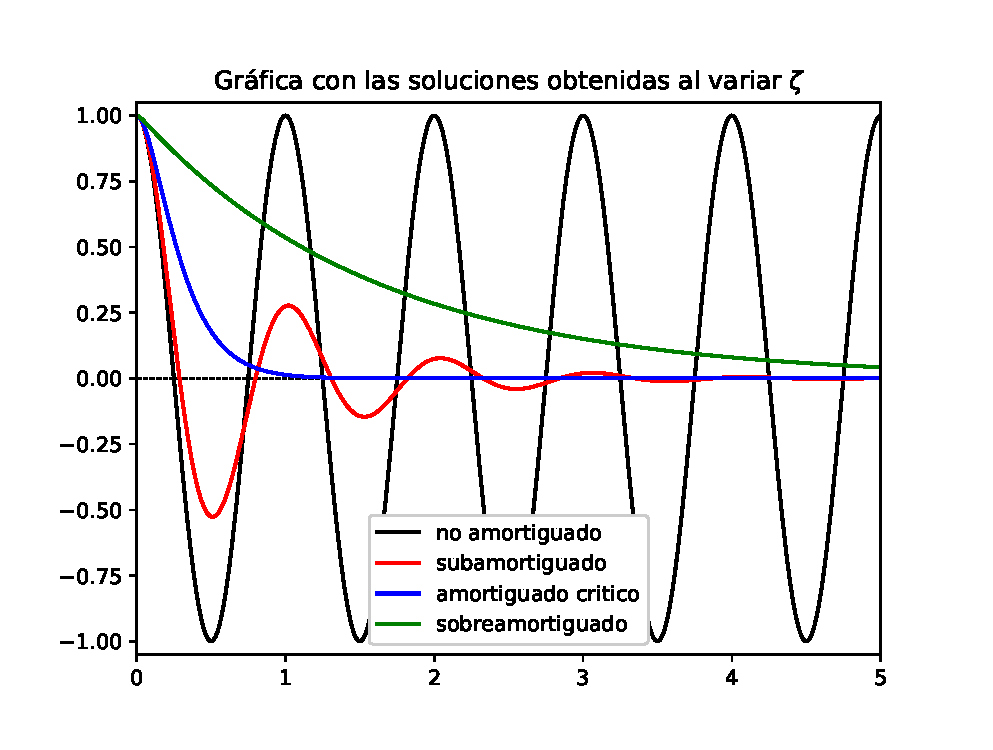
\includegraphics[scale=0.5]{Imagenes/ejercicio_odeint_02_oscilador_amortiguado.eps}
    \caption{Resultado obtenido al modificar el parámetro de amortiguamiento en la función \funcionazul{odeint}.}
\end{figure}
\end{frame}
\subsection{Circuito RLC}
\begin{frame}[plain]
\frametitle{Ejercicio 3 - Circuito RLC}
La corriente eléctrica de un circuito $RLC$ en serie, satisface la ecuación
\fontsize{12}{12}\selectfont
\begin{align}
L \, \dv{i}{t} + R \, i + \dfrac{1}{C} \, \int_{0}^{t} i(t^{\prime}) \dd{t^{\prime}} +\dfrac{1}{C} \, q(0) = E(t), \hspace{0.3cm} t > 0
    \label{eq:ecuacion1}
\end{align}
\begin{figure}[h!]
    \centering
    \includestandalone[scale=0.8]{Figuras/fig_edo_cto_RLC}
\end{figure}
\end{frame}
\begin{frame}
\frametitle{Circuito RLC}
\begin{figure}
    \centering
    \includestandalone[scale=0.7]{Figuras/fig_edo_cto_RLC}
\end{figure}
Cuando el circuito se cierra en el instante $t = 0$, se tiene que $i = i(t)$ es la corriente, $R$ es la resistencia, $L, C, E$ vienen dadas por: $L = \SI{200}{\henry}$, $C = \SI{0.001}{\farad}$, $E(t) = \SI{1}{\volt}$ para $t > 0$.
\end{frame}
\begin{frame}
\frametitle{Circuito RLC}
\begin{figure}
    \centering
    \includestandalone[scale=0.7]{Figuras/fig_edo_cto_RLC}
\end{figure}
Las condiciones iniciales son $q(0) = 0$ (carga inicial del condensador), $i(0) = 0$. 
\end{frame}
\begin{frame}
\frametitle{Resolver el problema}
Hay que calcular la corriente para $0 \leq t \leq 5$ segundos, así como el factor de amortiguamiento y la frecuencia de oscilación del circuito $RLC$ para los siguientes valores de resistencia:
\begin{enumerate}
\item $R = \SI{0}{\ohm}$
\item $R = \SI{50}{\ohm}$
\item $R = \SI{100}{\ohm}$
\item $R = \SI{300}{\ohm}$
\end{enumerate}
\end{frame}
\begin{frame}
\frametitle{Solución al ejercicio}
Si definimos
\begin{align}
q(t) = \int_{0}^{t^{\prime}} i(t^{\prime}) \: \dd{t^{\prime}}
\label{eq:ecuacion2}
\end{align}
para luego derivar la expresión anterior
\begin{align}
\dv{q(t)}{t} = i(t), \hspace{1.5cm} q(0)=0
\label{eq:ecuacion3}
\end{align}
\end{frame}
\begin{frame}
\frametitle{Solución al ejercicio}
Sustituimos en la ecuación inicial, para re-escribir
{\fontsize{12}{12}\selectfont
\begin{align}
\dv{i(t)}{t} = -\dfrac{R}{L} \: i(t) - \dfrac{1}{L \: C} \: q(t) + \dfrac{1}{L \: C} \: q(0) + \dfrac{E(t)}{L}, \: i(0) =  0 
\label{eq:ecuacion4}
\end{align}}
La ecuación (\ref{eq:ecuacion1}) se transformó en un sistema de dos EDO de primer orden: las ecuaciones (\ref{eq:ecuacion3}) y (\ref{eq:ecuacion4}).
\end{frame}
\begin{frame}[fragile]
\frametitle{Transformación para la solución}
Entonces ya contamos con un sistema de dos EDO1 para ocuparlas en la notación para la solución numérica:
\begin{verbatim}
F[0] = y[1]
F[1] = -(R/L)* y[1]-(1.0/(L*C))*y[0]+E/L
\end{verbatim}
\end{frame}
\begin{frame}[fragile, allowframebreaks, plain]
\begin{lstlisting}[caption=Código para resolver el circuito RLC, style=codigopython]
from numpy import zeros, array, linspace
from scipy.integrate import odeint

def F(y, t, R, L) : 
    C = 0.001
    E = 1.0
            
    F = zeros(2, dtype='floatA_64_B')
    F[A_0_B] = y[A_1_B]
    F[A_1_B] = -(R/L)*y[A_1_B] - (1.0/(L*C))*y[A_0_B] + E/L
    return F

t = linspace(0.0, 5.0, 200)
yA_0_B = array([0.0, 0.0])
h = 0.01

L = 200.0
R = [0.0, 50.0, 100.0, 500.0]

sol = odeint(....)
\end{lstlisting}
\end{frame}
\begin{frame}
\frametitle{Solución gráfica}
Ya contamos ahora con la solución, pero queremos que se ejecute el código una sola vez para que obtengamos una gráfica con las soluciones para diferentes valores de resistencia.
\\
\bigskip
\textbf{Ejercicio a cuenta:} modifica el código de tal manera que obtengas la gráfica con los cuatro valores de resistencia, ocupa el paso de argumentos extra: \funcionazul{args}.
\end{frame}
\begin{frame}[plain]    
\frametitle{Solución gráfica con valores de $R$ superpuestos}
\begin{figure}
    \centering
    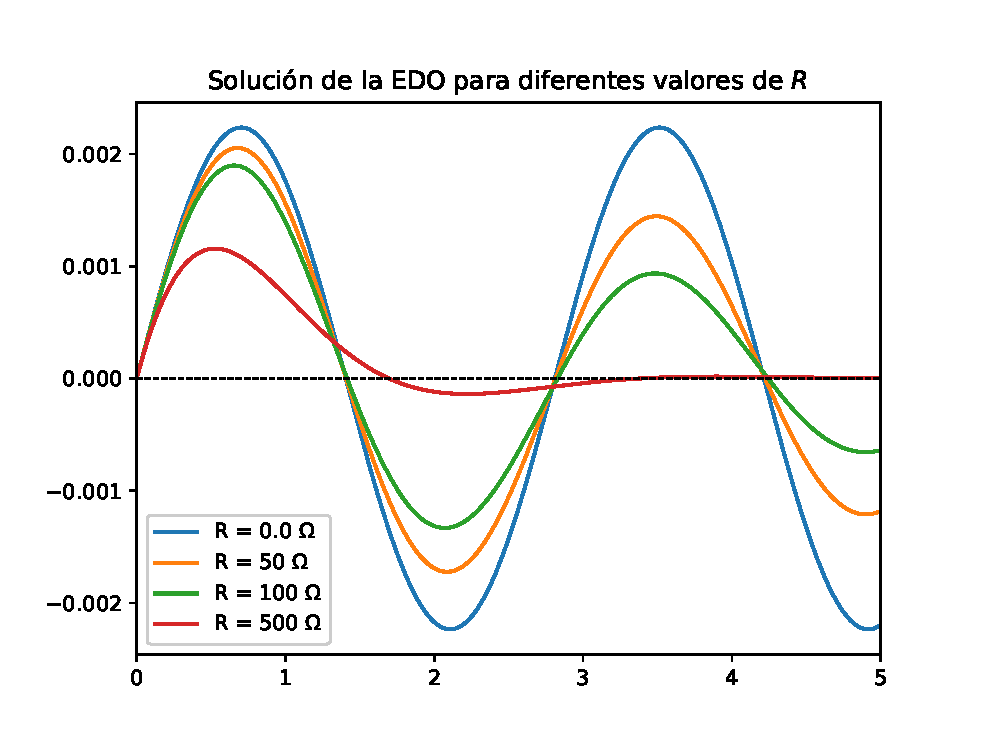
\includegraphics[scale=0.5]{Imagenes/ejercicio_odeint_03_circuito_RLC.eps}
    \caption{Gráfica que muestra el valor de la corriente para distintos valores de resistencia.}
\end{figure}
\end{frame}
\begin{frame}
\frametitle{\textbf{Ejercicio a cuenta}}
El enunciado nos pedía obtener el factor de amortiguamiento y la frecuencia de la señal obtenida para cada valor de $R$, así que hay que aplicarse para propocionar las respuestas pendientes.
\\
\bigskip
Deberás de responder haciendo un análisis con lo que ya sabes del curso de \emph{Electricidad}, ocupa lo necesario para ello. No esperamos que utilices funciones avanzadas de \python: transformadas de Fourier, etc.
\end{frame}
\subsection{Sistema de 3 masas acopladas}
\begin{frame}[fragile]
\frametitle{Ejercicio 4 - Masas acopladas}
En la figura se muestra un sistema de tres masas acopladas mediante resortes y amortiguadores.
\begin{figure}
    \centering
    \includestandalone[scale=0.75]{Figuras/fig_edo_sist_3_masas}
\end{figure}
\end{frame}
\begin{frame}[fragile]
\frametitle{Ejercicio 4 - Masas acopladas}
Los desplazamientos de estas tres masas satisfacen las ecuaciones dadas por:
\fontsize{12}{12}\selectfont
\begin{align*} 
M_{1} \: \stilde{y}_{1} + B_{1} \: \ptilde{y}_{1} + K_{1} \: y_{1} - B_{1} \: \ptilde{y}_{2} - K_{2} \: y_{2} &= F_{1}(t) \\
-B_{1} \: \ptilde{y}_{1} - K_{1} \: y_{1} + M_{2} \:  \stilde{y}_{2} + B_{1} \: \ptilde{y}_{2} + (K_{1} + K_{2}) \: y_{2} - K_{2} \: y_{3} &= 0 \\
- K_{2} \: y_{2} + M_{3} \: \stilde{y}_{3} + B_{2} \: \ptilde{y}_{3} + (K_{2} + K_{3})  \: y_{3} &=  F_{3}(t) 
\end{align*}
\begin{figure}[h!]
    \centering
    \includestandalone[scale=0.75]{Figuras/fig_edo_sist_3_masas}
\end{figure}
\end{frame}
\begin{frame}
\frametitle{Condiciones iniciales}
Las constantes y condiciones iniciales son
\fontsize{12}{12}\selectfont
\begin{tabbing}
$K_{1} = K_{2} = K_{3} = 1$ \hspace{1.2cm} \= (constantes de los resortes, $\si{\kilo\gram\meter\per\square\second}$) \\
$M_{1} = M_{2} = M_{3} = 1$ \> (masa, $\si{\kilo\gram}$) \\
$F_{1}(t) = 1, F_{3}(t) = 0$ \> (fuerza, $\si{\newton}$) \\
$B_{1} = B_{2} = 0.1$ \> (coeficientes de amortiguamiento, $\si{\kilo\gram\per\second}$) \\
$y_{1}(0) = \ptilde{y}_{1}(0) = y_{2}(0) = \ptilde{y}_{2}(0) = y_{3}(0) = \ptilde{y}_{3}(0) = 0$ \\
\> (condiciones iniciales)
\end{tabbing}
\end{frame}
\begin{frame}
\frametitle{Problema a resolver}
Resuelve el sistema para determinar la posición $y_{i}$ de cada masa en $0 \leq t \leq 60$ segundos, elabora una gráfica con las tres trayectorias.
\end{frame}
\begin{frame}
\frametitle{Antes de proponer un código}
Necesitamos manejar el sistema de las $3$ EDO2, de tal manera que podamos representar un sistema de $6$ EDO1, entonces consideremos el siguiente:
\\
\bigskip
Hint: Definiendo
\begin{align*}
y_{4} = \ptilde{y}_{1}, \hspace{1cm} y_{5} = \ptilde{y}_{2}, \hspace{1cm} y_{6} = \ptilde{y}_{3}
\end{align*}
\end{frame}
\begin{frame}
\frametitle{Antes de proponer un código}
Así, la ecuación inicial se escribe como \emph{un conjunto de seis EDO de primer orden}, de la siguiente manera:
\fontsize{12}{12}\selectfont
\begin{align*}
\ptilde{y}_{1} &= y_{4} \\
\ptilde{y}_{2} &= y_{5} \\
\ptilde{y}_{3} &= y_{6} \\
\ptilde{y}_{4} &= \left[ -B_{1} \: y_{4} - K_{1} \: y_{1} + B_{1} \: y_{5} + K_{2} \: y_{2} + F_{1} \right] / M_{1} \\
\ptilde{y}_{5} &= \left[ B_{1} \: y_{4} + K_{1} \: y_{1} - B_{1} \: y_{5} - \left( K_{1} + K_{2} \right) \: y_{2} + K_{2} \: y_{3} \right] / M_{2}\\
\ptilde{y}_{6} &= \left[ K_{2} \: y_{2} - B_{2} \: y_{6} - \left( K_{2} + K_{3} \right) \: y_{3} + F_{3} \right] / M_{3}
\end{align*}
\end{frame}
\begin{frame}[fragile, allowframebreaks, plain]
\begin{lstlisting}[caption=Código para el sistema de masas, style=codigopython]
def F(y, t) : 
    F = zeros(6, dtype='floatA_64_B')
    F[0] = y[3]
    F[1] = y[4]
    F[2] = y[5]
    F[3] = (-0.1*y[3] - y[0] + 0.1*y[4] + y[1] + 1.)
    F[4] = (0.1*y[3] + y[0] - 0.1*y[4] - 2.*y[1] + y[2])
    F[5] = (y[1] - 0.1*y[5] - 2.*y[2])
    return F

t = linspace(0, 61, 100)
yA_0_B = array([0., 0., 0., 0., 0., 0.])

sol = odeint(F, yA_0_B, t)
\end{lstlisting}
\end{frame}
\begin{frame}
\frametitle{Problema a cuenta}
Deberás de incorporar una rutina de gráficación para mostrar el resultado que nos devuelve la función \funcionazul{odeint}.
\\
\bigskip
En la siguiente figura se puede ver el desplazamiento para cada masa.
\end{frame}
\begin{frame}[plain]
\frametitle{Solución al problema}
\begin{figure}
    \centering
    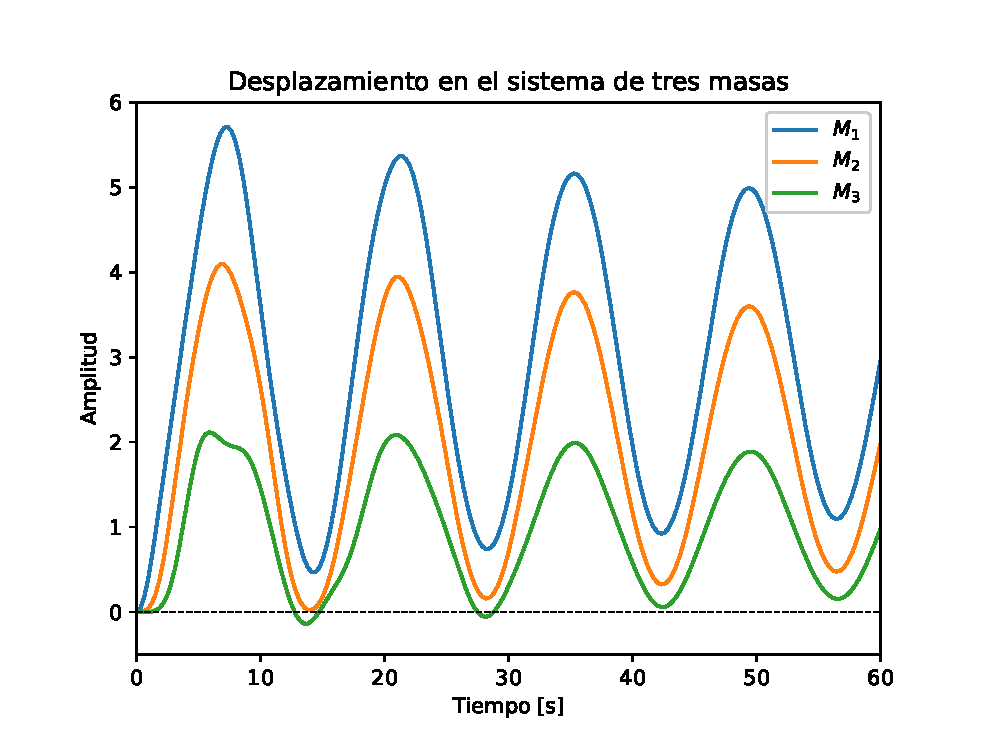
\includegraphics[scale=0.5]{Imagenes/ejercicio_odeint_04_sistema_3masas.eps}
    \caption{Se describe el desplazamiento para cada una de las masas.}
\end{figure}
\end{frame}
\subsection{Sistema Lotka-Volterra}
\begin{frame}
\frametitle{Ejercicio 5 - Sistema Lotka-Volterra}
Las ecuaciones de Lotka-Volterra, también son conocidas como \emph{ecuaciones de depredador-presa}.
\\
\bigskip
Está descrito por un sistema de 2 ecuaciones diferenciales no lineales de primer orden.
\end{frame}
\begin{frame}
\frametitle{Sistema Lotka-Volterra}
Se utiliza frecuentemente para describir la dinámica de sistemas biológicos donde interaccionan dos especies: un depredador y una de sus presas.
\end{frame}
\begin{frame}
\frametitle{Sistema de ecuaciones acopladas}
El sistema evoluciona de acuerdo al par de ecuaciones:
\begin{align*}
\dv{u}{t} &= a \: u - b \: u \: v \\
\dv{v}{t} &= -c \: v + d \: b\: u\: v
\end{align*}
donde:  
\setbeamercolor{item projected}{bg=yellow!80!black,fg=black}
\setbeamertemplate{enumerate items}[circle]
\begin{enumerate}[<+->]
\item $u$ es el número de presas (ej. Conejos)
\item $v$ es el número de depredadores (ej. Zorros)
\seti
\end{enumerate}
\end{frame}
\begin{frame}
\frametitle{Sistema de ecuaciones acopladas}
\begin{align*}
\dv{u}{t} &= a \: u - b \: u \: v \\
\dv{v}{t} &= -c \: v + d \: b\: u\: v
\end{align*}
donde:
\setbeamercolor{item projected}{bg=yellow!80!black,fg=black}
\setbeamertemplate{enumerate items}[circle]
\begin{enumerate}[<+->]
\conti
\item $a$ es la tasa natural de crecimiento de conejos, sin que haya zorros.
\item $b$ es la tasa natural de la muerte de conejos, debido a la depredación.
\seti
\end{enumerate}
\end{frame}
\begin{frame}
\frametitle{Sistema de ecuaciones acopladas}
\begin{align*}
\d{u}{t} &= a \: u - b \: u \: v \\
\d{v}{t} &= -c \: v + d \: b\: u\: v
\end{align*}
donde:
\setbeamercolor{item projected}{bg=yellow!80!black,fg=black}
\setbeamertemplate{enumerate items}[circle]
\begin{enumerate}[<+->]
\conti
\item $c$ es la tasa natural de la muerte del zorro, cuando no hay conejos.
\item $d$ es el factor que describe el número de conejos capturados.
\end{enumerate}
\end{frame}
\begin{frame}
\frametitle{Poblaciones iniciales}
Vamos a utilizar $X = [u, v]$ para describir el estado de las poblaciones.
\\
\bigskip
A continuación veremos en cada diapositiva una parte del código, que deberás de conjuntar en un solo archivo.
\end{frame}
\begin{frame}[allowframebreaks, plain, fragile]
\frametitle{Definiendo las ecuaciones}
\begin{lstlisting}[caption=Código inicial, style=codigopython]
import numpy as np

a = 1.
b = 0.1
c = 1.5
d = 0.75

def dXdt(X, t = 0):
    return np.array([ a*X[0] - b*X[0]*X[1], -c*X[1] + d*b*X[0]*X[1]])
\end{lstlisting}
\end{frame}
\begin{frame}[allowframebreaks, plain, fragile]
\frametitle{Población en equilibrio}
Antes de usar la función \funcionazul{odeint} para integrar el sistema, veremos de cerca la posición de equilibrio.
\\
\bigskip
El equilibrio ocurre cuando \emph{la tasa de crecimiento es igual a $0$}, lo que nos da dos puntos fijos:
\begin{lstlisting}[caption=Equilibrio en las poblaciones, style=codigopython]
XfA_0_B = np.array([0., 0.])
XfA_1_B = np.array([ c/(d * b), a/b])

all(dXdt(XfA_0_B) == np.zeros(2)) and all(dXdt(XfA_1_B) == np.zeros(2))
\end{lstlisting}
\end{frame}
\begin{frame}[allowframebreaks, fragile]
\frametitle{Sobre la función \funcionazul{all}}
La función \funcionazul{all()} recibe un objeto iterable y retorna \funcionazul{True} si todos sus elementos son verdaderos:
\begin{verbatim}
>>> all([True, False])
False

>>> all([True, True])
True

>>> all(["Hola mundo!", None])
False

>>> all([1, 2, 3])
True

>>> all([0, 1, 2, 3])
False
\end{verbatim}
\end{frame}
\begin{frame}[fragile]
\frametitle{Variable temporal y cond. iniciales}
Para usar la función \funcionazul{odeint}, hay que definir el parámetro de tiempo $t$, así como las condiciones inciales de la población: $10$ conejos y $5$ zorros.
\end{frame}
\begin{frame}[fragile]
\frametitle{Variable temporal y cond. iniciales}
\begin{lstlisting}[caption=Código para las condiciones iniciales, style=codigopython]
t = np.linspace(0, 15, 500)
              
XA_0_B = np.array([10.0, 5.0])         
            
X = odeint(dXdt, XA_0_B, t)
conejos, zorros = X.T
\end{lstlisting}
\end{frame}
\begin{frame}[fragile]
\frametitle{Para graficar el resultado}
En la última instrucción para obtener la solución, se ha utilizado: \verb|conejos, zorros = X.T|, que lo que hace es tomar el arreglo \funcionazul{X} y hacer la transposición, de tal manera que podemos ocupar ahora con una variable \funcionazul{conejos} y en otras \funcionazul{zorros}, los valores de esos arreglos.
\end{frame}
\begin{frame}
\frametitle{Ejercicio a cuenta}
Tendrás que incorporar la rutina de graficación y obtener:
\begin{figure}[h!]
    \centering
    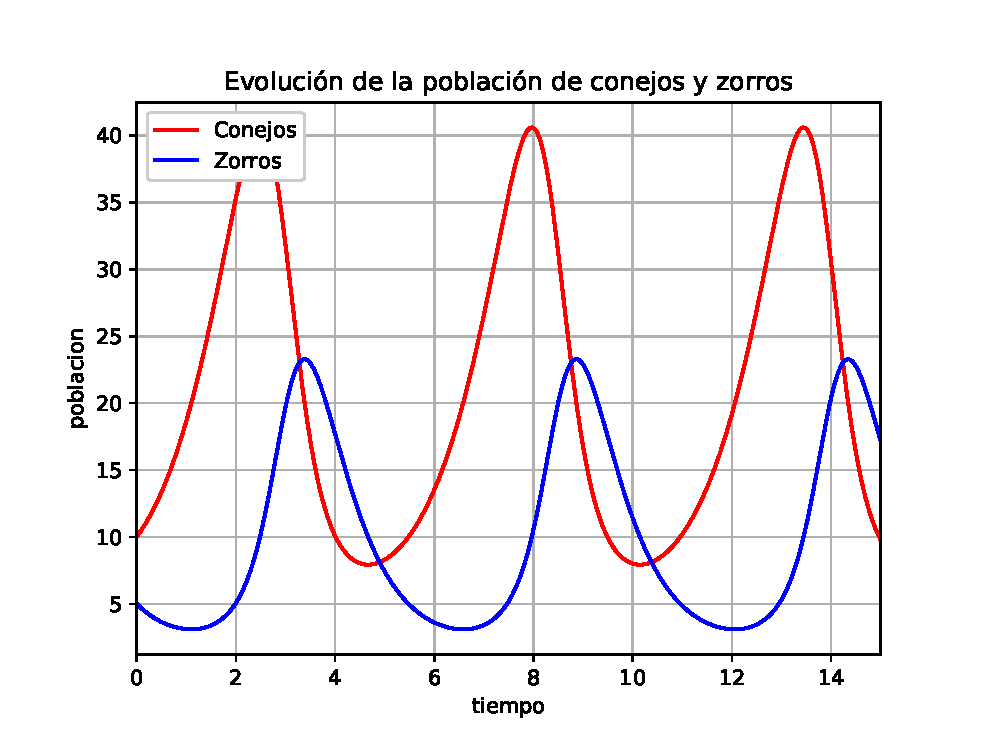
\includegraphics[scale=0.5]{Imagenes/ejercicio_odeint_05_sistema_lotka-volterra_01.eps} 
\end{figure}
\end{frame}
\begin{frame}
\frametitle{Interpretación de la solución}
De la gráfica vemos que se da un crecimiento de conejos, mientras desciende el número de zorros, pero luego ambas especies aumentan su población.
\\
\bigskip
Hay un pico en la población de conejos, pero al aumentar la población de zorros, el número de conejos va disminuyendo.
\end{frame}
\begin{frame}
\frametitle{Intepretación de la solución}
Al haber un descenso en el número de conejos, comienza una competencia por el alimento de los zorros por lo que algunos mueren y desciende la población.
\\
\bigskip
Al haber menos zorros, se permite que el número de conejos comience a elevarse y se repite de manera cíclica este comportamiento.
\end{frame}
% \begin{frame}
% \frametitle{Graficando la solución}
% Una vez obtenido el código para la solución del problema, ahora nos corresponde graficar el conjunto de datos obtenido:
% \end{frame}
% \begin{frame}[fragile, plain, allowframebreaks]
% \frametitle{Graficando la solución}
% \begin{lstlisting}[caption=Código para graficar, style=FormattedNumber, basicstyle=\linespread{1.1}\ttfamily=\small, columns=fullflexible]
% conejos, zorros = X.T

% f_1_ = plt.figure()
% plt.plot(t, conejos, 'r-', label='Conejos')
% plt.plot(t, zorros  , 'b-', label='Zorros')
% plt.grid()
% plt.legend(loc='best')
% plt.xlabel('tiempo')
% plt.ylabel('poblacion')
% plt.title('Evolucion de la poblacion de conejos y zorros')
% plt.show()
% \end{lstlisting}
% \end{frame}
% \begin{frame}[plain]
% \frametitle{Resultado gráfico}
% \begin{figure}
%     \centering
%     \includegraphics[scale=0.6]{Imagenes/LotkaVolterra_01.eps} 
% \end{figure}
% \end{frame}
\begin{frame}
\frametitle{Interpretación de la solución}
En resumen: la gráfica anterior nos da la información sobre el número tanto de conejos como de zorros durante el intervalo de tiempo estudiado, es decir, tenemos una especie de \enquote{censo} durante la observación.
\end{frame}
\begin{frame}
\frametitle{Extendiendo la interpretación}
Para ver la \emph{dinámica de las poblaciones} propiamente, ahora graficamos el espacio fase del sistema, por lo que tenemos que hacer algunos ajustes en el código que usamos anteriormente.
\\
\bigskip
Los elementos visuales que agregaremos, básicamente son \enquote{decoradores}, con los cuales tendremos una gráfica mucho más completa y sencilla de interpretar. Puedes extender la revisión de cada función en la documentación oficial de \python.
\end{frame}
\begin{frame}[fragile]
\frametitle{El módulo \texttt{color map}}
El módulo \funcionazul{cm} (\texttt{color map}) proporciona un conjunto de mapas de colores predeterminados, así como las funciones necesarias para crear nuevos mapas de color. Lo ocuparemos a modo de presentar un gradiente de tonalidad.
\\
\bigskip
Existen varios mapas ya definidos: \funcionazul{autumn, bone, cool, copper, flag, gray, hot, hsv, jet, pink, prism, spring, summer, winter, spectral}.
\end{frame}
\begin{frame}[fragile]
\frametitle{Elementos adicionales para la gráfica}
Necesitamos una tupla de valores para crear ese gradiente, por ello ocupamos en las variables \funcionazul{values} y en \funcionazul{vcolors}, un arreglo con valores, nótese que en la variable \funcionazul{vcolors}, usaremos el mapa \funcionazul{autumn}.
\begin{verbatim}
values  = linspace(0.3, 0.9, 5)                         

vcolors = plt.cm.autumn_r(linspace(0.3, 1.,
            len(values)))  
\end{verbatim}
\end{frame}
\begin{frame}[fragile]
\frametitle{La función \texttt{zip}}
Ocuparemos la función \funcionazul{zip}: es una función incorporada de \python, es decir, no necesita importarse.
\\
\bigskip
Toma como argumento dos o más objetos iterables (idealmente cada uno de ellos con la misma cantidad de elementos) y devuelve un nuevo iterable cuyos elementos son tuplas que contienen un elemento de cada uno de los iteradores originales.
\end{frame}
\begin{frame}[fragile]
\frametitle{La función \texttt{zip}}
Ejemplo del manejo de la función \funcionazul{zip}:
\begin{lstlisting}[caption=Ejemplo de la función zip, style=codigopython]
paises = ["China", "India", "Estados Unidos", "Indonesia"]
poblaciones = [1391, 1364, 327, 264]
mezcla = list(zip(paises, poblaciones))
print(mezcla)
\end{lstlisting}
\fontsize{12}{12}\selectfont
[('China', 1391), ('India', 1364), ('Estados Unidos', 327), ('Indonesia', 264)]
\end{frame}
\begin{frame}[allowframebreaks, fragile]
\frametitle{Curvas de nivel}
Se van a dibujar ahora las trayectorias (\emph{curvas de nivel}) para diferentes condiciones iniciales (número de conejos y zorros)
\begin{lstlisting}[caption=Graficando las curvas de nivel, style=codigopython]
for v, col in zip(values, vcolors):
    XA_0_B = v * XfA_1_B
    
    X = odeint( dXdt, XA_0_B, t)

    plt.plot( X[:,0], X[:,1], lw=3.5*v, color=col, label='XA_0_B=(%.f, %.f)' % ( XA_0_B[0], XA_0_B[1]) )
\end{lstlisting}
En cada gráfica se modificará el grosor de la línea y el color que se le asocia.
\end{frame}
\begin{frame}
\frametitle{Resultado parcial}
\fontsize{12}{12}\selectfont
Presentamos la gráfica que se obtiene con el procedimiento anterior
\begin{figure}[h!]
    \centering
    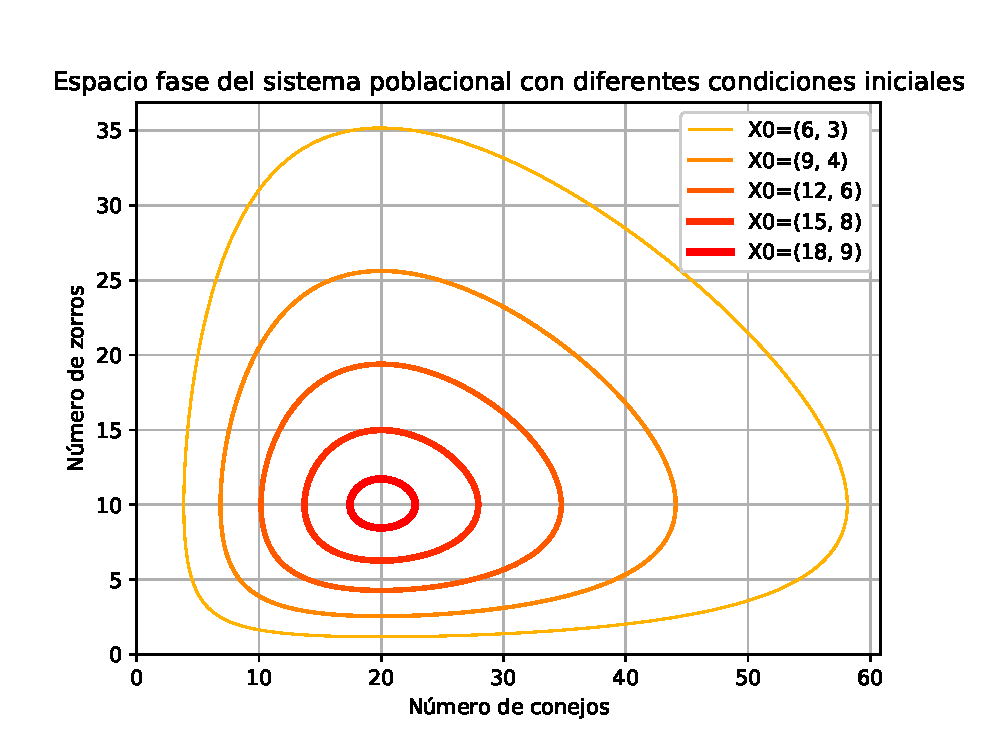
\includegraphics[scale=0.4]{Imagenes/ejercicio_odeint_05_sistema_lotka-volterra_02.eps}
    \caption{Espacio fase del sistema poblacional de conejos y zorros.}
\end{figure}
\end{frame}
\begin{frame}
\frametitle{Sobre el espacio fase}
Vemos de la gráfica anterior que para cada condición inicial, tenemos un comportamiento cerrado. Vemos el número de conejos en función del número de zorros, a lo largo del tiempo.
\\
\bigskip
Pero aún así, podemos obtener más información sobre la dinámica que existe en el sistema, para ello, tendremos que ajustar nuevamente la parte de graficación.
\end{frame}
\begin{frame}
\frametitle{Campo vectorial de direcciones}
Podemos mostrar también el campo de direcciones de las ecuaciones.
\\
\bigskip
Simplificando de tal manera que el tamaño de las flechas esté normalizado para que todas tengan la misma longitud y darles un color para representar su módulo.
\end{frame}
\begin{frame}
\frametitle{Dos funciones de \texttt{numpy}}
Para lo anterior, vamos a necesitar dos funciones adicionales:
\setbeamercolor{item projected}{bg=blue!70!black,fg=yellow}
\setbeamertemplate{enumerate items}[circle]
\begin{enumerate}[<+->]
\item La función \funcionazul{numpy.meshgrid}
\item La función \funcionazul{numpy.hypot}
\end{enumerate}
\end{frame}
\begin{frame}
\frametitle{La función \texttt{numpy.meshgrid}}
Esta función devuelve una lista de arreglos de coordenadas a partir de vectores de coordenadas.
\\
\bigskip
Veamos un ejemplo: supongamos que queremos definir un área en dos dimensiones formada por los puntos de coordenadas $x = 0, 1, 2$ e $y = 0, 1, 2$:
\end{frame}
\begin{frame}
\frametitle{La función \texttt{numpy.meshgrid}}
Conjunto de coordenadas $x$ e $y$:
\begin{figure}[h!]
    \centering
    \includestandalone[scale=1.3]{Figuras/funcion_meshgrid}
    \caption{Conjunto de $9$ puntos.}
\end{figure}
\end{frame}
\begin{frame}
\frametitle{La función \texttt{numpy.meshgrid}}
Como se ve en figura anterior, los conjuntos de coordenadas $x$ e $y$ definen $9$ puntos cuyas coordenadas en el plano se muestran en rojo.
\\
\bigskip
El objetivo es obtener dos arreglos, cada uno de tamaño $(3, 3)$ en los que se incluyan por separado las coordenadas $x$ e $y$ de los $9$ puntos en cuestión.
\end{frame}
\begin{frame}
\frametitle{La función \texttt{numpy.meshgrid}}
Esto es exactamente lo que hace la función \funcionazul{numpy.meshgrid}: acepta como entrada las coordenadas que definen el segmento del hiperplano (puede tratarse de dos dimensiones o de cualquier otro número de ellas) y devuelve arreglos con las coordenadas de dichos puntos:
\end{frame}
\begin{frame}[fragile]
\frametitle{La función \texttt{numpy.meshgrid}}
Si definimos
\begin{verbatim}
coord_x = [0, 1, 2]
coord_y = [0, 1, 2]
x, y = np.meshgrid(coord_x, coord_y)
\end{verbatim}
\end{frame}
\begin{frame}[fragile]
\frametitle{La función \texttt{numpy.meshgrid}}
Visualizamos las variables $x$, $y$, entonces la salida será:
\fontsize{12}{12}\selectfont
\begin{verbatim}
print(x)
[[0 1 2]
[0 1 2]
[0 1 2]]

print(y)
[[0 0 0]
 [1 1 1]
 [2 2 2]]
\end{verbatim}
\end{frame}
\begin{frame}[allowframebreaks, fragile]
\frametitle{Definición de una malla}
Se define una malla sobre nuestro espacio de solución:
\begin{lstlisting}[caption=Creando una malla, style=codigopython]
ymax = plt.ylim(ymin = 0)[1]
xmax = plt.xlim(xmin = 0)[1]

nbpoints   = 20

x = np.linspace(0, xmax, nbpoints)
y = np.linspace(0, ymax, nbpoints)

XA_1_B, YA_1_B  = np.meshgrid(x, y)
\end{lstlisting}
\end{frame}
\begin{frame}
\frametitle{La función \texttt{numpy.hypot}}
La función \funcionazul{hypot} calcula la hipotenusa de un triángulo rectángulo, dado un lado y la perpendicular.
\\
\bigskip
El valor que devuelve es equivalente a
\begin{align*}
\sqrt{x_{1}^{2} + x_{2}^{2}}
\end{align*}
\end{frame}
\begin{frame}[fragile]
\frametitle{Calculando la magnitud del vector}
\begin{lstlisting}[caption=Magnitud del vector y su dirección, style=codigopython]
DXA_1_B, DYA_1_B = dXdt([XA_1_B, YA_1_B])                      

M = (np.hypot(DXA_1_B, DYA_1_B))                           

M[ M == 0] = 1.                                 

DXA_1_B /= M                                        
DYA_1_B /= M
\end{lstlisting}
\end{frame}
\begin{frame}[fragile]
\frametitle{Calculando la magnitud del vector}
\setbeamercolor{item projected}{bg=yellow!80!black,fg=black}
\setbeamertemplate{enumerate items}[circle]
\begin{enumerate}[<+->]
\item Con \funcionazul{X1} y \funcionazul{Y1} se crea una malla. 
\item Con \funcionazul{DX1} y \funcionazul{DY1} se calcula el crecimiento de las poblaciones en la malla.
\item Con la variable \funcionazul{M} se calcula la norma de la tasa de crecimiento, usando la función \funcionazul{hypot}.
\item La expresión \funcionazul{M[M==0]=1.} evita que tengamos una división entre cero.
\item Con la operación \funcionazul{DX1/M} y \funcionazul{DY1/M} se normaliza cada vector.
\end{enumerate}
\end{frame}
\begin{frame}[fragile]
\frametitle{La función \texttt{quiver}}
Necesitarmos la función \funcionazul{quiver} para mostrar la gráfica del campo vectorial, como flechas con componentes $(u, v)$ en los puntos ($x, y)$
\\
\medskip
\verb|quiver(x, y, u, v)|
\\
\medskip
Entonces veremos al vector como flechas en las coordenadas especificadas por cada par de elementos $(x, y)$. Puedes revisar en la documentación de \funcionazul{matplotlib} el uso de más argumentos.
\end{frame}
\begin{frame}[plain, allowframebreaks, fragile]
\frametitle{Dibujando las direcciones del vector}
Se dibujan las direcciones usando \funcionazul{quiver}
\begin{lstlisting}[caption=Dibujando las direcciones del vector resultante, style=codigopython]
plt.title('Trayectorias y campo de direccion')

Q = plt.quiver(XA_1_B, YA_1_B, DXA_1_B, DYA_1_B, M, pivot='mid', cmap=plt.cm.jet)
\end{lstlisting}
\end{frame}
\begin{frame}[fragile]
\frametitle{La función \texttt{quiver}} 
La función \funcionazul{quiver} genera el mapa vectorial, requiere de siete argumentos (al menos para el ejercicio): las posiciones \funcionazul{X1}, \funcionazul{Y1} de inicio, el valor de las componentes del vector \funcionazul{DX1}, \funcionazul{DY1} y el color asociado \funcionazul{cmap}, el argumento \funcionazul{pivot} indica en qué parte del punto de la malla se va a colocar el vector.
\end{frame}
\begin{frame}[plain]
\frametitle{Resultado gráfico completo}
\begin{figure}[h!]
    \centering
    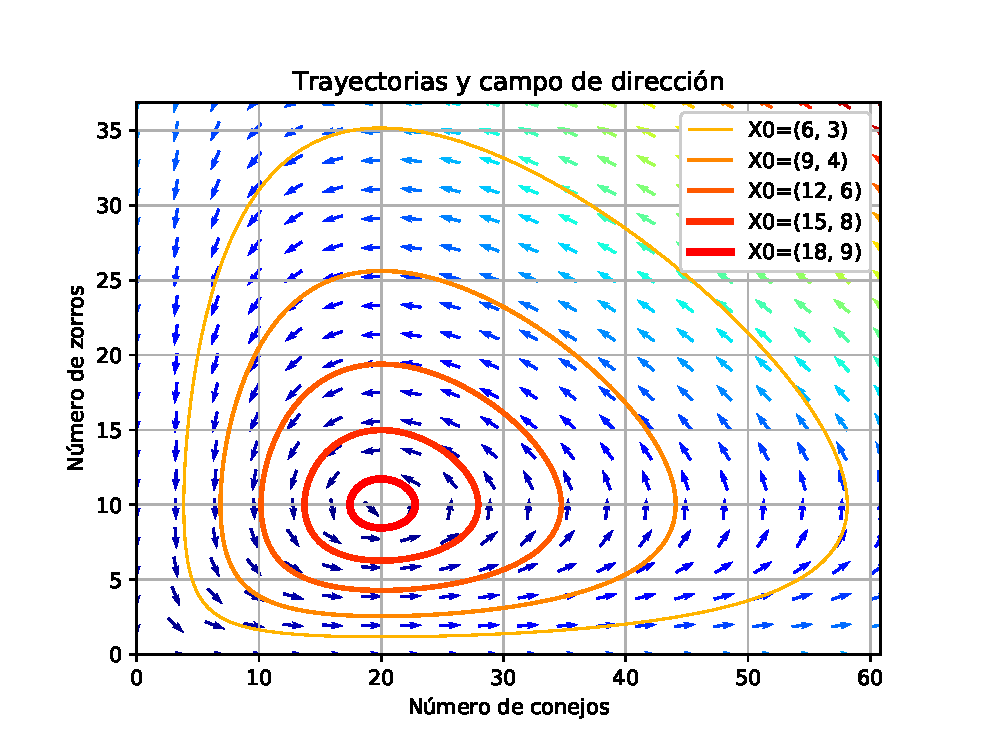
\includegraphics[scale=0.5]{Imagenes/ejercicio_odeint_05_sistema_lotka-volterra_03.eps} 
\end{figure}
\end{frame}
\begin{frame}
\frametitle{¿Qué nos dice la gráfica?}
Si nos fijamos en una de las líneas continuas, la coordenada $x$ en cada punto indica el número de presas y la coordenada $y$ el número de depredadores.
\end{frame}
\begin{frame}
\frametitle{¿Qué nos dice la gráfica?}
La evolución a lo largo del tiempo que hemos representado antes, se obtiene al recorrer esta curva en sentido antihorario.
\\
\bigskip
Podemos ver también como el campo de direcciones nos señala la tendencia del sistema en cada situación.
\end{frame}
\begin{frame}
\frametitle{¿Qué nos dice la gráfica?}
Por ejemplo, una flecha que apunta hacia arriba a la derecha indica que con ese número de conejos y zorros en nuestro sistema, la tendencia será que aumenten ambos.
\end{frame}
\begin{frame}
\frametitle{Ejercicio a cuenta}
El \emph{modelo de Lorenz} se usa para estudiar la formación de torbellinos en la atmósfera, aunque abordó el problema de manera general, estableció las bases para el estudio de sistemas dinámicos.
\end{frame}
\begin{frame}
\frametitle{Ejercicio para resolver}
El conjunto de ecuaciones está dado por
\begin{align*}
\dv{y_{1}}{t} &= a(y_{2} - y_{1}) \\[0.5em]
\dv{y_{2}}{t} &= (b - y_{3}) \: y_{1} - y_{2} \\[0.5em]
\dv{y_{3}}{t} &= y_{1} \: y_{2} - c \: y_{3} \\[0.5em]
y_{1}(0) = y_{2}(0) = y_{3}(0) = 1
\end{align*}
en el modelo $a$, $b$ y $c$ son parámetros positivos. 
\end{frame}
\begin{frame}
\frametitle{Ejercicio para resolver}
Resuelve este modelo numéricamente y grafica la solución.
\\
\bigskip
Utiliza los siguientes valores $a = 10$, $b = 28$ y $c =8/3$. Interpreta la solución.
\end{frame}
\begin{frame}[plain]
\frametitle{Gráfica de la solución}
\begin{figure}
    \centering
    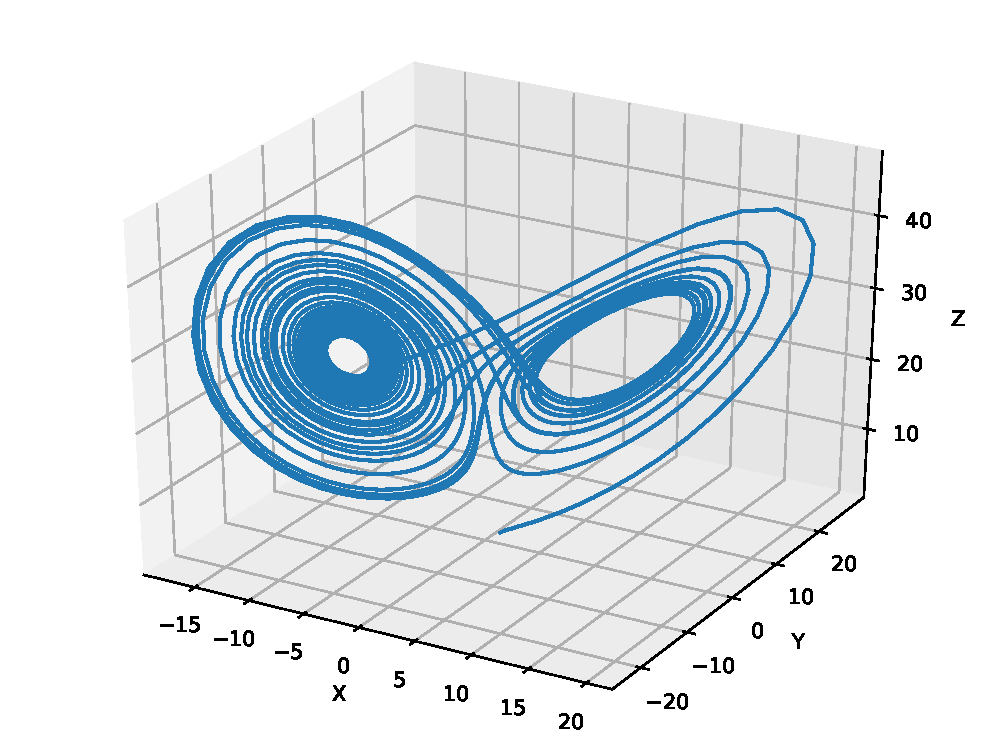
\includegraphics[scale=0.5]{Imagenes/ejercicio_odeint_06_sistema_lorenz.eps} 
\end{figure}
\end{frame}
\begin{frame}
\frametitle{Repite el ejercicio}
Repite el ejercicio modificando el valor de $c=6./3$. Vuelve a graficar e interpreta de nuevo el resultado obtenido.
\end{frame}
% \begin{frame}[fragile]
% \frametitle{Para generar una gráfica 3D}
% Para graficar una función de tres variables en \funcionazul{matplotlib}, debemos de utilizar una combinación de dos librerías:
% \begin{verbatim}
% import matplotlib.pyplot as plt
% import mpl_toolkits.mplot3d.axes3d as p3
% \end{verbatim}    
% \end{frame}
% \begin{frame}[fragile]
% \frametitle{Usando \texttt{plot3D}}
% Hay un importante cambio cuando graficamos tres variables con \funcionazul{matplotlib}, hay adecuar el espacio de trabajo mediante la siguiente referencia:
% \begin{verbatim}
% fig = plt.figure()

% ax = p3.Axes3D(fig)
% \end{verbatim}
% Con \texttt{plt} definimos el espacio común de graficación, pero con \texttt{ax}, ahora y contamos con la manera de usar la graficación de tres variables.
% \end{frame}
% \begin{frame}[fragile]
% \frametitle{La función \texttt{plot3D}}
% La función \funcionazul{plot3D} ocupa los argumentos de la misma manera que \funcionazul{plot}, por lo que debemos de usar la sintaxis:
% \begin{verbatim}
% ax.plot3D(x, y, z)

% ax.set_xlabel('X')
% ax.set_ylabel('Y')
% ax.set_zlabel('Z')

% fig.add_axes(ax)
% plt.show()
% \end{verbatim}
% \end{frame}
% \section{Métodos Multipaso}
% \frame{\tableofcontents[currentsection, hideothersubsections]}
% \subsection{Método de Numerov}
% \begin{frame}
% \frametitle{Método de Numerov}
% Un problema de valores iniciales para una EDO2 tiene la forma:
% \begin{align}
% \dv[2]{y}{x} = f(x) \, y + g(x)
% \label{eq:ecuacion_12_61}
% \end{align}
% \pause
% sin la primera derivada y el lado derecho depende linealmente de la solución, este tipo de EDO2 se pueden resolver de manera más eficiente utilizando el \textoazul{método de varios pasos} desarrollado por el astrónomo B. Numerov.
% \end{frame}
% \begin{frame}
% \frametitle{Características del método}
% El \textoazul{método de Numerov} debe su popularidad a su:
% \setbeamercolor{item projected}{bg=blue!70!black,fg=yellow}
% \setbeamertemplate{enumerate items}[circle]
% \begin{enumerate}[<+->]
% \item Alta precisión del orden $\order{h^{6}}$.
% \item Simplicidad algorítmica (implementación)
% \item Aplicación directa para resolver la ecuación de Schrödinger, como ecuación fundamental de la mecánica de ondas.
% \end{enumerate}
% \end{frame}
% \begin{frame}
% \frametitle{Versatilidad del método}
% Pasando a una notación vectorial, el \textoazul{método de Numerov} se vuelve igualmente adecuado para resolver sistemas de EDO2.
% \\
% \bigskip
% Cabe destacar que con una metodología similar a la que se describe a continuación también es aplicable para obtener integradores para sistemas de EDO de orden superior que solo involucran derivadas de orden par.
% \end{frame}
% \subsection*{Construcción del método}
% \begin{frame}
% \frametitle{Construcción del método}
% En la primera etapa, considerando que la solución $y$ tiene el grado necesario de suavidad (\emph{derivadas continuas hasta el quinto orden}) y tomando como referencia su valor $y_{m}$ en algún punto $x_{m}$, se pueden expresar los valores en $x_{m+h}$ y, respectivamente, en $x_{m-h}$ por la serie Taylor:
% \end{frame}
% \begin{frame}
% \frametitle{Construcción del método}
% \begin{align*}
% y_{m+1} &= y_{m} + h \, \ptilde{y}_{m} + \dfrac{1}{2!} \, h^{2} \, \stilde{y}_{m} + \\
% &+ \dfrac{1}{3!} \, h^{3} \, \ntilde{y}{3}_{m} + \dfrac{1}{4!} \, h^{4} \, \ntilde{y}{4}_{m} + \dfrac{1}{5!} \, h^{5} \, \ntilde{y}{5}_{m} + \order{h^{6}} \\[0.5em]
% y_{m-1} &= y_{m} - h \, \ptilde{y}_{m} + \dfrac{1}{2!} \, h^{2} \, \stilde{y}_{m} + \\
% &- \dfrac{1}{3!} \, h^{3} \, \ntilde{y}{3}_{m} + \dfrac{1}{4!} \, h^{4} \, \ntilde{y}{4}_{m} - \dfrac{1}{5!} \, h^{5} \, \ntilde{y}{5}_{m} + \order{h^{6}}
% \end{align*}
% \end{frame}
% \begin{frame}
% \frametitle{Construcción del método}
% Las derivadas impares se pueden eliminar sumando las expresiones anteriores:
% \begin{align}
% y_{m+1} + y_{m-1} =  2 \, y_{m} + h^{2} \, \stilde{y}_{m} + \dfrac{1}{12} \, h^{4} \, \ntilde{y}{4}_{m} + \order{h^{6}}
% \label{eq:ecuacion_12_62}
% \end{align}
% \end{frame}
% \begin{frame}
% \frametitle{Construcción del método}
% De hecho, al buscar una relación algebraica para la solución propagada $y_{m + 1}$ en términos de valores anteriores, es necesario reemplazar las derivadas restantes $\stilde{y}_{m}$ e $\ntilde{y}{4}_{m}$, con esquemas de diferencias finitas, sin embargo, se preserva la exactitud del orden $\order{h^{6}}$
% \end{frame}
% \begin{frame}
% \frametitle{Construcción del método}
% La segunda derivada $\stilde{y}_{m}$ se toma propiamente de la ecuación diferencial:
% \begin{align}
% \stilde{y}_{m} = f_{m} \, y_{m} + g_{m}
% \label{eq:ecuacion_12_63}
% \end{align}
% donde $f_{m} \equiv f(x_{m})$ y $g_{m} \equiv g(x_{m})$.
% \end{frame}
% \begin{frame}
% \frametitle{Construcción del método}
% Para la derivada de cuarto orden $\ntilde{y}{4}_{m}$ se puede ver como la segunda derivada de $\stilde{y}_{m}$, y de nuevo, tomando la ecuación diferencial, tenemos que
% \begin{align}
% \ntilde{y}{4}_{m} = \big[ f(x) \, y + g(x) \stilde{\big]}_{m}
% \label{eq:ecuacion_12_64}
% \end{align}
% \end{frame}
% \begin{frame}
% \frametitle{Construcción del método}
% Para las segundas derivadas, en general, se puede diseñar un esquema de diferencias finitas al mantener la aproximación de orden $\order{h^{4}}$ en la ecuación (\ref{eq:ecuacion_12_62}):
% \begin{align*}
% h^{2} \, \stilde{y}_{m} = y_{m+1} - 2 \, y_{m} + y_{m-1} + \order{h^{4}}
% \end{align*}
% \end{frame}
% \begin{frame}
% \frametitle{Construcción del método}
% Aplicando en particular este esquema a
% \begin{align*}
% \big[ f(x) \, y + g(x) \stilde{\big]}_{m}
% \end{align*}
% la ecuación (\ref{eq:ecuacion_12_64}) cambia a
% \begin{align}
% \begin{aligned}
% h^{4} \, \ntilde{y}{4}_{m} &= h^{2} + \big( f_{m+1} \, y_{m+1} - 2 \, f_{m} \, y_{m} + f_{m-1} \, y_{m-1} \big) + \\
% &+ h^{2} \big( g_{m+1} + 10 \, g_{m} + g_{m-1} \big) + \order{h^{6}}
% \end{aligned}
% \label{eq:ecuacion_12_65}
% \end{align}
% \end{frame}
% \subsection*{Fórmula de Numerov}
% \begin{frame}
% \frametitle{Fórmula de Numerov}
% Al incorporar las ecs. (\ref{eq:ecuacion_12_63}) y (\ref{eq:ecuacion_12_65}) en la ec. (\ref{eq:ecuacion_12_62}), para luego agrupar términos, obtenemos la \emph{fórmula de Numerov}:
% \begin{align}
% \begin{aligned}
% y_{m+1} &= \left[ \left( 2 + \dfrac{5}{6} \, h^{2} \, f_{m} \right) \, y_{m} - \left( 1 - \dfrac{1}{12} \, h^{2} \, f_{m-1} \right) \, y_{m-1} + \right. \\[0.5em]
% &\left. + \dfrac{1}{12} h^{2} \big( g_{m+1} + 10 \, g_{m} + g_{m-1} \big) \right] \times \\[0.5em]
% &\times \left( 1 - \dfrac{1}{12} \, h^{2} \, f_{m+1} \right)^{-1} + \order{h^{6}}
% \end{aligned}
% \label{eq:ecuacion_12_66}
% \end{align}
% \end{frame}
% \begin{frame}
% \frametitle{Fórmula de Numerov}
% Al definir las cantidades auxiliares
% \begin{align}
% u_{m} = 1 - \dfrac{1}{12} \, h^{2} \, f_{m}
% \label{eq:ecuacion_12_67}
% \end{align}
% La \textoazul{fórmula de Numerov} se puede expresar de manera más conveniente, dada por:
% \end{frame}
% \begin{frame}
% \frametitle{Fórmula de Numerov}
% \begin{align}
% \begin{aligned}
% y_{m+1} &= \dfrac{(12 - 10 \, u_{m}) \, y_{m} - u_{m-1} \, y_{m-1}}{u_{m+1}} + \\[0.5em]
% &+ \dfrac{1}{12} \, h^{2} \, \dfrac{g_{m+1} + 10 \, g_{m} + g_{m-1}}{u_{m+1}} + \order{h^{6}}
% \end{aligned}
% \label{eq:ecuacion_12_68}
% \end{align}
% \end{frame}
% \subsection*{Desventaja del método}
% \begin{frame}
% \frametitle{Desventaja del método}
% La desventaja del método Numerov es que no se inicia automáticamente, lo que está intrínsecamente relacionado con su naturaleza de varios pasos.
% \\
% \bigskip
% En consecuencia, se deben proporcionar dos valores de solución iniciales antes de que se pueda iniciar la recurrencia (ec. \ref{eq:ecuacion_12_68}).
% \end{frame}
% \begin{frame}
% \frametitle{Resolviendo la desventaja}
% Esto se puede lograr mediante un paso inicial realizado con un algoritmo de inicio automático (\textoazul{Euler-Cromer}, \textoazul{Runge-Kutta}, etc.), en el caso de aplicaciones especialmente exigentes, utilizando la expansión Taylor de la solución, con particularidades integradas de la EDO.
% \end{frame}
% \begin{frame}
% \frametitle{Resolviendo la desventaja del método}
% El \textoazul{método Numerov} no es adecuado para implementaciones cerradas de uso general.
% \\
% \bigskip
% Con el objetivo de una codificación eficiente, es preferible aprovechar la forma particular de las funciones $f (x)$ y $g (x)$ para generar adecuadamente los dos valores iniciales necesarios para iniciar el algoritmo.
% \end{frame}
% \begin{frame}
% \subsection*{Aplicación del método}
% \frametitle{Ejemplo: Ec. de Schrödinger}
% Consideremos la ecuación de Schrödinger indepediente del tiempo en una dimensión para una partícula de masa $\mu$ bajo un potencial $V(x)$:
% \begin{align}
% - \dfrac{\hbar^{2}}{2 \, \mu} \, \dv[2]{\psi}{x} + V(x) \, \psi(x) = E \, \psi (x)
% \label{eq:ecuacion_12_69}
% \end{align}
% \end{frame}
% \begin{frame}
% \frametitle{Ejemplo: Ec. de Schrödinger}
% La ecuación se puede simplificar al hacer un cambio adimensional:
% \begin{align}
% \stilde{\psi} = 2 \, \big[ V(x) - E(x) \big] \, \psi
% \label{eq:ecuacion_12_70}
% \end{align}
% \pause
% Por lo que podemos presentar las expresiones que definen la solución en términos del \textoazul{método de Numerov}:
% \end{frame}
% \begin{frame}
% \frametitle{Solución con el método de Numerov}
% Las expresiones son:
% \begin{align}
% u_{m} &= 1 - \dfrac{1}{6} h^{2} \big[ V(x_{m}) - E \big] \label{eq:ecuacion_12_71} \\[0.5em]
% \psi_{m+1} &= \dfrac{(12 - 10 \, u_{m}) \, \psi_{m} - u_{m-1} \, \psi_{m-1}}{u_{m+1}} \label{eq:ecuacion_12_72}
% \end{align}
% \end{frame}
% \begin{frame}
% \frametitle{Código para el método}
% La implementación del \textoazul{método de Numerov} como solución a problemas de tipo Cauchy para la ecuación de onda (\ref{eq:ecuacion_12_70}), se presenta a continuación:
% \end{frame}
% \begin{frame}[allowframebreaks, fragile]
% \frametitle{Código para el método de Numerov}
% \begin{lstlisting}[caption=Código para el método de Numerov, style=codigopython]
% def Numerov(E, V, x, y, nx, yA_0_B, dyA_0_B):
%     hx = x[2] - x[1]
%     y[1] = yA_0_B; dy = dyA_0_B
 
%     dA_2_By = 2e0 * (V[1] - E) * y[1]
%     dy += hx * dA_2_By
%     y[2] = y[1] + hx * dy
 
%     hA_6_B = hx*hx/6e0
%     umA_1_B = 1e0 - hA_6_B * (V[1] - E)
%     um  = 1e0 - hA_6_B * (V[2] - E)
%     for m in range(2, nx):
%        upA_1_B = 1e0 - hA_6_B * (V[m+1] - E)
%        y[m+1] = ((12e0 - 10e0*um) * y[m] - um1 * y[m-1]) / upA_1_B
%        umA_1_B = um; um = upA_1_B
 
%        if (abs(y[m+1]) > 1e10): break
 
%     return m
% \end{lstlisting}
% \end{frame}
% \subsection*{Sobre el código}
% \begin{frame}
% \frametitle{Sobre el código}
% Suponiendo que la energía potencial que se recibirá está tabulada en el arreglo \funcionazul{V}, la rutina \funcionazul{Numerov} propaga la solución \funcionazul{y}, para una energía dada \funcionazul{E}, comenzando desde los valores iniciales \funcionazul{y0} y \funcionazul{dy0} sobre \funcionazul{nx} puntos equidistantes de la malla.
% \end{frame}
% \begin{frame}
% \frametitle{Sobre el código}
% Para comenzar correctamente la recurrencia con \emph{dos valores de solución}, se realiza un paso inicial de \textoazul{Euler-Cromer} para calcular la solución en el segundo punto de malla.
% \end{frame}
% \begin{frame}
% \frametitle{Sobre el código}
% No es necesario asignar un arreglo completo a los valores auxiliares $u_{m}$ (dependiendo de los valores del potencial local), ya que se usan un triplete y se almacenan como una pila de tres variables: \funcionazul{um1}, \funcionazul{um} y \funcionazul{up1}, correspondientes a $u_{m-1}$, $u_{m}$ y $u_{m+1}$.
% \\
% \bigskip
% Se reducen en cada paso al actualizar el componente más avanzado: \funcionazul{up1}.
% \end{frame}
% \begin{frame}
% \frametitle{Cuidado con el manejo del código}
% Para muchas aplicaciones, es esencial identificar las regiones en donde la solución posiblemente comience a divergir numéricamente.
% \end{frame}
% \begin{frame}
% \frametitle{Cuidado con el manejo del código}
% De hecho, para potenciales y soluciones de rango infinito en donde se espera que desaparezcan asintóticamente, es muy probable que más allá de una región donde la solución se vuelve insignificante y satisface el comportamiento asintótico, comienza a crecer, sobrecargado por la acumulación de errores de truncamiento y redondeo.
% \end{frame}
% \begin{frame}
% \frametitle{Cuidado con el manejo del código}
% Prácticamente, en el caso de soluciones divergentes donde
% \begin{align*}
% \abs{\psi (x)} > \num{e10}
% \end{align*}
% la propagación se detiene y el índice del punto de divergencia: \funcionazul{m}, se devuelve junto con la solución al programa de llamada para tomar otras medidas o acciones.
% \end{frame}
% \begin{frame}
% \frametitle{Completando el ejercicio}
% El \textoazul{método de Numerov} se ejemplifica en la siguiente sección junto con el llamado \enquote{método de disparo} para determinar los estados ligados de la ecuación de onda de Schrödinger.
% \end{frame}
% \section{Métodos Indirectos}
% \frame{\tableofcontents[currentsection, hideothersubsections]}
% \subsection{Método de disparo}
% \begin{frame}
% \frametitle{Repaso}
% Hasta este punto, hemos discutido solo métodos para resolver \emph{problemas de valores iniciales}, para los cuales las condiciones que complementan la EDO se especifican en un solo punto.
% \end{frame}
% \begin{frame}
% \frametitle{Método de disparo}
% Estos métodos relativamente fáciles de usar siguen demostrando su utilidad cuando se trata de \emph{problemas de valores en dos puntos}, siempre que estén contenidos en el denominado \enquote{algoritmo de disparo}.
% \end{frame}
% \begin{frame}
% \frametitle{Método de disparo}
% Esencialmente, un \textoazul{método de disparo} transforma un problema de dos puntos en un problema de valores iniciales e intenta, a modo de prueba y error, reproducir la segunda condición de límite \emph{(no utilizada)}.
% \end{frame}
% \begin{frame}
% \frametitle{Método de disparo}
% Consideremos el problema general de dos puntos de segundo orden con las \emph{condiciones de frontera de tipo Dirichlet} (valor fijo):
% \begin{align}
% \dv[2]{y}{x} &= f(x, y, \ptilde{y}) \label{eq:ecuacion_12_73} \\[0.5em]
% y(x_{a}) &= y_{a} \hspace{0.75cm} y(x_{b}) = y_{b} \label{eq:ecuacion_12_74}
% \end{align}
% donde suponemos que la solución $y(x)$ y la primera derivada $\ptilde{y}(x)$ son funciones continuas.
% \end{frame}
% \begin{frame}
% \frametitle{De la primera derivada}
% La derivada $\ptilde{y}(x_{a}) = \ptilde{y}_{a}$ en la frontera izquierda del intervalo, no se conoce \emph{a priori}, pero se \textbf{se define de manera unívoca} en las condiciones de frontera.
% \end{frame}
% \begin{frame}
% \frametitle{De la primera derivada}
% Suponemos que $\ptilde{y}_{a}$ se conoce desde el inicio, por lo que el problema de dos puntos se puede sustituir por un problema equivalente de valores iniciales:
% \begin{align}
% \dv[2]{y}{x} &= f(x, y, \ptilde{y}) \label{eq:ecuacion_12_75} \\[0.5em]
% y(x_{a}) &= y_{a} \hspace{0.75cm} \ptilde{y}(x_{a}) = \ptilde{y}_{a}
% \end{align}
% teniendo la misma solución y satisfaciendo también la segunda condición de frontera que no se está usando: $y(x_{b}) = y_{b}$
% \end{frame}
% \begin{frame}
% \frametitle{Revisión de la solución}
% Supongamos que comenzamos la propagación de la solución, en lugar de la primera derivada verdadera (desconocida) $\ptilde{y}_{a}$, con un par de derivadas de prueba, $\ptildosargs{y}{1}_{a} < \ptildosargs{y}{2}_{a}$, y que obtenemos correspondientemente, dos diferentes soluciones del problema, para las cuales los valores en el punto final $x_{b}$ son $y_{b}^{(1)}$ y respectivamente, $y_{b}^{(2)}$.
% \end{frame}
% \begin{frame}
% \frametitle{Revisión de los signos}
% Si tanto $y_{b}^{(1)}$ como, $y_{b}^{(2)}$ mantienen el mismo signo del valor final verdadero $y_{b}$, en virtud de la continuidad de la solución, se deduce que la derivada verdadera $\ptilde{y}_{a}$ no está contenida entre los valores de prueba iniciales $\ptildosargs{y}{1}_{a}$  y $\ptildosargs{y}{2}_{a}$. 
% \end{frame}
% \begin{frame}
% \frametitle{Revisión de los signos}
% Por el contrario, si $y_{b}^{(1)}$ e $y_{b}^{(2)}$ están en diferentes lados de $y_{b}$, se deduce que $\ptilde{y}_{a}$ está ubicado entre $\ptildosargs{y}{1}_{a}$  y $\ptildosargs{y}{2}_{a}$, o sucede que:
% \begin{align}
% \left( y_{b}^{(1)} - y_{b} \right) \left( y_{b}^{2} - y_{b} \right) &> 0 \Rightarrow \ptilde{y}_{a} \notin \left[ \ptildosargs{y}{1}_{a}, \ptildosargs{y}{2}_{a} \right] \label{eq:ecuacion_12_77} \\[0.5em]
% \left( y_{b}^{(1)} - y_{b} \right) \left( y_{b}^{2} - y_{b} \right) &\leq 0 \Rightarrow \ptilde{y}_{a} \in \left[ \ptildosargs{y}{1}_{a}, \ptildosargs{y}{2}_{a} \right] \label{eq:ecuacion_12_78}
% \end{align}
% \end{frame}
% \begin{frame}
% \frametitle{Usando cálculo de raíces}
% En una estrategia de \emph{separación y refinación de raíces}:
% \setbeamercolor{item projected}{bg=blue!70!black,fg=yellow}
% \setbeamertemplate{enumerate items}[circle]
% \begin{enumerate}
% \item En el primer caso, uno no usaría el intervalo actual y pasaría a un nuevo intervalo de prueba $\left[ \ptildosargs{y}{1}_{a}, \ptildosargs{y}{2}_{a} \right]$.
% \seti
% \end{enumerate}
% \end{frame}
% \begin{frame}
% \frametitle{Usando cálculo de raíces}
% \setbeamercolor{item projected}{bg=blue!70!black,fg=yellow}
% \setbeamertemplate{enumerate items}[circle]
% \begin{enumerate}
% \conti
% \item En el segundo caso, uno refinaría iterativamente la derivada e implícitamente, la solución, aplicando una bisección el intervalo de prueba $\left[ \ptildosargs{y}{1}_{a}, \ptildosargs{y}{2}_{a} \right]$, hasta el intervalo objetivo $ \left[ y_{b}^{(1)}, y_{b}^{(2)} \right]$ entre corchetes el verdadero valor final $y_{b}$ disminuiría por debajo de una tolerancia predefinida.
% \end{enumerate}
% \end{frame}
% \subsection*{Código método de disparo}
% \begin{frame}
% \frametitle{Código para el método de disparo}
% La rutina \funcionazul{Disparo} se muestra a continuación, veamos que  recibe una malla $x$ completa a través del arreglo \funcionazul{x}, junto con los valores límite \funcionazul{ya} e \funcionazul{yb}, los límites \funcionazul{dy1} y \funcionazul{dy2} del intervalo de búsqueda para la primera derivada, y la tolerancia \funcionazul{eps}, dentro del cual se espera que la solución encontrada cumpla con el valor límite \funcionazul{yb}.
% \end{frame}
% \begin{frame}
% \frametitle{Código para el método de disparo}
% Para las propagaciones repetidas de \funcionazul{x[1]} a \funcionazul{x[nx]} que requiere el algoritmo de disparo, la rutina \funcionazul{Disparo} llama a la función auxiliar \funcionazul{Propag}, que es un simple propagador genérico basado en el \textoazul{método Euler-Cromer}.
% \end{frame}
% \begin{frame}
% \frametitle{Código para el método de disparo}
% La rutina \funcionazul{Disparo} inicialmente realiza dos propagaciones completas para las derivadas de entrada, \funcionazul{dy1} y \funcionazul{dy2}, y compara las desviaciones de solución correspondientes, \funcionazul{f1} y \funcionazul{f2}, del valor límite deseado \funcionazul{yb}.
% \end{frame}
% \begin{frame}
% \frametitle{Código para el método de disparo}
% Si \funcionazul{f1} y \funcionazul{f2} tienen el mismo signo, el intervalo entre \funcionazul{dy1} y \funcionazul{dy2} ciertamente no contiene la derivada inicial buscada y la rutina devuelve un \funcionazul{dy} falso y el indicador \funcionazul{exist} queda en $0$.
% \end{frame}
% \begin{frame}
% \frametitle{Código para el método de disparo}
% Por el contrario, si las dos soluciones de prueba se desvían en diferentes lados de \funcionazul{yb} (\funcionazul{f1} y \funcionazul{f2} tienen signos opuestos), la rutina inicia el refinamiento iterativo del intervalo entre \funcionazul{dy1} y \funcionazul{dy2} por el \textoazul{método de bisección}.
% \end{frame}
% \begin{frame}
% \frametitle{Código para el método de disparo}
% En cada paso de reducción a la mitad, la rutina \funcionazul{Disparo} comienza la propagación con la derivada promedio anterior y mantiene como derivadas iniciales de frontera, aquellas que conducen a desviaciones finales de signos opuestos y, que, obviamente, llevan entre corchetes a la derivada exacta.
% \end{frame}
% \begin{frame}
% \frametitle{Código para el método de disparo}
% La capacidad de agrupar la derivada exacta, duplicada por su solidez algorítmica y simplicidad, son precisamente las características beneficiosas que recomiendan el \textoazul{método de bisección}.
% \end{frame}
% \begin{frame}[allowframebreaks, fragile]
% \frametitle{Código en \python}
% \begin{lstlisting}[caption=Código para el método de disparo, style=codigopython]
% from math import fabs
% from Metodos_Directos import EulerCromerA_1_B

% def Propag(x, y, nx, yA_0_B, dyA_0_B, Func):
%     hx = x[2] - x[1]
%     y[1] = yA_0_B; dy = dyA_0_B
%     for m in range(1,nx):
%         (y[m+1], dy) = EulerCromerA_1_B(x[m], hx, y[m], dy, Func)


% def Disparo(x, y, nx, ya, yb, dyA_1_B, dyA_2_B, eps, Func):
%     itmax = 100

%     Propag(x, y, nx, ya, dyA_1_B, Func)
%     fA_1_B = y[nx] - yb
%     Propag(x, y, nx, ya, dyA_2_B, Func)
%     fA_2_B = y[nx] - yb

%     if (fA_1_B*fA_2_B < 0):
%         exist = 1
%         for it in range(1,itmax+1):
%             dy = 0.5e0*(dyA_1_B + dyA_2_B)
%             Propag(x, y, nx, ya, dy, Func)
%             f = y[nx] - yb
%             if (fA_1_B*f > 0): dyA_1_B = dy
%             else:          dyA_2_B = dy
%             if (fabs(f) <= eps): break

%         if (it >= itmax): print("Metodo Disparo: se ha rebasado el numero maximo de bisecciones!!")
%     else:
%         dy = 1e10; exist = 0

%     return (dy, exist)
% \end{lstlisting}
% \end{frame}
% \subsection*{Primer ejemplo}
% \begin{frame}
% \frametitle{Primer ejemplo}
% Para revisar el \textoazul{método de disparo}, consideramos a continuación el cálculo de los polinomios de Legendre, $P_{n} (x)$, a partir de su ecuación diferencial.
% \\
% \bigskip
% El correspondiente problema de valores de frontera de dos puntos, que cumple con la estandarización comúnmente utilizada $P_{n} (1) = 1$, puede escribirse como
% \end{frame}
% \begin{frame}
% \frametitle{Definición de $P_{n}(x)$}
% La EDO2 que define los $P_{n}(x)$ es
% \begin{align}
% \dv[2]{P_{n}}{x} &= \dfrac{1}{1 - x^{2}} \, \left[ 2 \, x \, \dv{P_{n}}{x} - n (n + 1) \, P_{n} \right] \label{eq:ecuacion_12_79} \\[0.5em]
% P_{n}(-1) &= (-1)^{n}, \hspace{0.75cm} P_{n}(1) = 1 \label{eq:ecuacion_12_80}
% \end{align}
% \end{frame}
% \begin{frame}
% \frametitle{Propiedad de los polinomios}
% Hacemos un uso explícito de la paridad bien definida de los polinomios de Legendre, teniendo en cuenta su carácter alternativamente simétrico y antisimétrico (determinado por la independencia de la EDO en el signo de $x$), el dominio de integración puede reducirse desde $[-1,1]$ a $[0, 1]$
% \end{frame}
% \begin{frame}
% \frametitle{Propiedad de los polinomios}
% En este contexto, se puede demostrar que la derivada en el origen: $P_{n} (0)$, que puede ser útil para la comparación con resultados numéricos, satisface la relación simple:
% \begin{align*}
% \ptilde{P}_{n}(0) = n \, P_{n-1} (0)
% \end{align*}
% \end{frame}
% \begin{frame}
% \frametitle{Uso de las condiciones iniciales}
% Por lo tanto, al detallar las condiciones iniciales que se utilizarán en $x = 0 $ para soluciones pares e impares, los polinomios de Legendre pueden considerarse como soluciones del problema de Cauchy:
% \begin{align}
% \stilde{y} &= \dfrac{1}{1 - x^{2}} \, \big[ 2 \, x \, \ptilde{y} - n (n + 1) \, y \big] \label{eq:ecuacion_12_81} \\[0.5em]
% y(0) &= y_{a} \hspace{0.5cm} \ptilde{y}(0) = 0, \hspace{0.5cm} n = 0, 2, \ldots \label{eq:ecuacion_12_82} \\[0.5em]
% y(0) &= 0 \hspace{0.5cm} \ptilde{y}(0) = \ptilde{y}_{a}, \hspace{0.5cm} n = 1, 3, \ldots \label{eq:ecuacion_12_83}
% \end{align}
% \end{frame}
% \begin{frame}
% \frametitle{Restricción adicinal}
% Además debemos de considerar la restricción adicional:
% \begin{align}
% y(1) = 1
% \label{eq:ecuacion_12_84}
% \end{align}
% \end{frame}
% \begin{frame}
% \frametitle{Propiedad de la ecuación}
% La homogeneidad de la ecuación de Legendre garantiza que cualquier solución multiplicada por una constante también es una solución. 
% \end{frame}
% \begin{frame}
% \frametitle{Propagación con valor inicial}
% De manera correspondiente, incluso para $n$ pares, el procedimiento equivale a la propagación directa de \emph{un valor inicial arbitrario} $\tilde{y} (0) = y_{a}$, que se finaliza reescalando la solución encontrada, $\tilde{y}(x)$, con el valor final $\tilde{y}(1)$, es decir, $y (x) = \tilde{y}(x) / \tilde{y}(1)$.
% \end{frame}
% \begin{frame}
% \frametitle{Condición no utilizada}
% De tal manera, la condición de límite no utilizada $y (1) = 1$, se cumple claramente.
% \\
% \bigskip
% En cuanto a las soluciones $n$ impares, requieren la aplicación real del método de disparo, lo que implica el cálculo de la derivada inicial correcta $\ptilde{y}_{a}$ mediante bisecciones iterativas en el intervalo $(-\infty, +\infty)$.
% \end{frame}
% \begin{frame}
% \frametitle{Condiciones para el ejercicio}
% Se hará el cálculo para los polinomios de Legendre mediante el \textoazul{método de disparo}, para $n=5$, con un paso de integración $h=\num{e-4}$ y una tolerancia de $\varepsilon = \num{e-4}$.
% \end{frame}
% \begin{frame}
% \frametitle{Operación del código}
% Para el valor límite $y(1)$, el código determina la derivada inicial refinada $\ptilde{y} (0) = 1.8768$, en lugar del valor exacto $\ptilde{P}_{5} (0) = 15/8 = 1.875$.
% \end{frame}
% \begin{frame}
% \frametitle{Operación del código}
% El error local máximo con respecto a la solución exacta asciende a $\num{4.3e-4}$ y se espera que sea más alto que $\varepsilon$ (que se refiere solo al valor límite).
% \\
% \bigskip
% Obviamente, la concordancia con el resultado exacto se puede mejorar reduciendo el tamaño del paso de integración.

% La figura 12.7 muestra dos soluciones de prueba que resultan para las derivadas iniciales particulares y (1) a = 1.5 e y (2) a = 2.5, que entrelazan la derivada exacta (P5 (0) = 1.875). Se puede ver que las soluciones de prueba bordean la solución exacta (P5 (x)), similar a la forma en que los valores finales correspondientes y (1) by e (2) b encierran el verdadero valor límite yb.

% Si bien se clasifica entre los algoritmos más adecuados para los problemas de valor límite para las EDO, el método de disparo sin duda muestra todo su potencial cuando se aplica a problemas de valor propio y, además, cuando se definen en dominios infinitos. Estos dos aspectos de modelado adicionales requieren un tratamiento numérico específico. Uno de los ejemplos prototípicos de esta categoría son los problemas de estado límite para la ecuación 1D Schrödinger independiente del tiempo.
% \end{frame}

\end{document}